\documentclass[10pt,twoside]{report}
\usepackage[utf8]{inputenc}
\usepackage[dutch]{babel}
\usepackage{multicol}
\usepackage{float}
\usepackage[a4paper, margin=0.98in]{geometry}
\usepackage[fleqn]{amsmath}
\usepackage{amsfonts}
\usepackage{titling}
\usepackage{sectsty}
\usepackage{pgfplots}
\usepackage{pgfplotstable}
\usepackage{multirow}
\usepackage{hyperref}
\usepackage{makecell}
\usepackage{fancyhdr}
\usepackage{minted}
\usepackage{biblatex}
\usepackage{mathtools}
\usepackage[toc,page]{appendix}
\usepackage{longtable}
\usepackage{scrextend, perpage}
\usepackage[ruled]{manyfoot}
\usepackage{lastpage}
\usepackage{rotating, graphicx}
\usepackage{wrapfig}

% footer defs
\DeclareNewFootnote{A}

\MakePerPage{footnote}

\def\resetfootnotemarks{%
  \deffootnote[1em]{0em}{1em}{$^{\alph{footnote}}$}%
  \deffootnotemark{\textsuperscript{\alph{footnote}}}%
}
\resetfootnotemarks

\newcommand\footdef[3]{%
  \deffootnotemark{\textsuperscript{\thefootnotemark}}%
  \setcounter{footnoteA}{#1}%
  \addtocounter{footnoteA}{-1}%
  \setbox0=\hbox{#2$^{\thefootnotemark}$:\ }%
  \deffootnote[\wd0]{0em}{1em}{#2$^{\thefootnotemark}$:\ }%
  #2\footnoteA{#3}%
  \resetfootnotemarks%
}

\newcommand\footdefmark[2]{%
  \deffootnotemark{\textsuperscript{\thefootnotemark}}%
  #2\footnotemark[#1]%
  \deffootnotemark{\textsuperscript{\alph{footnote}}}%
}

% inf symbol
\def\infinity{\rotatebox{90}{8}}

% bibliography management
\addbibresource{bronnen.bib}

\pgfplotsset{compat=newest}

% Header sizes
\sectionfont{\fontsize{11}{14}\selectfont}
\subsectionfont{\fontsize{10}{13}\selectfont}
\subsubsectionfont{\fontsize{9}{12}\selectfont}

% colors
\definecolor{Earth}{rgb}{0.368417,0.506779,0.709798}
\definecolor{Garnet}{rgb}{0.880722,0.611041,0.142051}
\definecolor{Opal}{rgb}{0.560181,0.691569,0.194885}
\definecolor{Sapphire}{rgb}{0.922526,0.385626,0.209179}
\definecolor{Steel}{rgb}{0.528488,0.470624,0.701351}
\definecolor{Sunrise}{rgb}{0.772079,0.431554,0.102387}
\definecolor{codegray}{gray}{0.9}

% Header and footers
\pagestyle{fancy}
\fancyhf{}

% Title page
\author{Laurens Ketsman}
\title{Automatisering van zuur-base titraties}
\date{17 januari 2017}

% Section numbering
\setcounter{secnumdepth}{5}

% Graphics path
\graphicspath{{img/}}

% minted code style
\usemintedstyle{vs}

% custom commands
\newcommand{\overbar}[1]{\mkern 1.5mu\overline{\mkern-1.5mu#1\mkern-1.5mu}\mkern 1.5mu}

% add blank pages
\newcommand\blankpage{%
    \null
    \thispagestyle{empty}%
    \addtocounter{page}{-1}%
    \newpage}

% inline code
\newcommand{\code}[1]{{\texttt{#1}}}

\begin{document}

\clearpage\maketitle
\thispagestyle{empty}

\blankpage

\tableofcontents
\thispagestyle{empty}

\newpage
\section*{Voorwoord}
\thispagestyle{empty}

% apply fancyhdr to chapter pages
\fancypagestyle{plain}{%
  \fancyhf{}%
    \fancyhead[RO]{\leftmark\ \rule[-0.25em]{0.14em}{1.3em}\ \thepage}
    \fancyhead[LE]{\thepage\ \rule[-0.25em]{0.14em}{1.3em}\ \rightmark}
}

\fancyfoot{}
\fancyhead[RO]{\leftmark\ \rule[-0.25em]{0.14em}{1.3em}\ \thepage}
\fancyhead[LE]{\thepage\ \rule[-0.25em]{0.14em}{1.3em}\ \rightmark}

\newpage
\chapter{Titraties achtergrond}

\chapter{Arduino Ontwerp}
\section{Wat is een Arduino?}
Arduino is een volledig platform van open-source hardware\footnote{Hardware waarvan het hardware design volledig open en beschikbaar is zodat anderen het kunnen namaken of uitbreidingen op kunnen voortbouwen.}. Voornamelijk is het een kleine maar veelzijdige microcontroller\footnote{Een kleine computer op 1 printplaat.} die volledig programmeerbaar en uit te breiden is.
\\\\
Het grote voordeel van een Arduino is dat deze relatief goedkoop is maar wel een grote flexibiliteit en vooral veelzijdigheid bied voor die prijs. Er zijn teveneens ook veel uitbreidingen en documentatie beschikbaar wat het een nummer 1 keuze maakt voor doe-het-zelf projecten.
\\\\
In dit project zullen we gebruikmaken van de Arduino UNO rev3.\\
Deze beschikt over:
\begin{itemize}
    \item 1 USB connectie voor seriële communicatie met de microcontroller
    \item 14 Digitale pins waarvan 6 met PWM\footnote{Pulse width modulation}
    \item 6 analoge pins
    \item 1 ATmega328P 16MHz controller
    \item 32KB flash geheugen
\end{itemize}
Volledige specificaties kunnen teruggevonden worden op de Arduino site\footnote{\url{www.arduino.cc/en/Main/ArduinoBoardUno}} of in de bijlagen.
\section{Waar worden Arduinos gebruikt?}
Arduinos worden vaak gebruikt door individuen voor hun projecten waar automatisatie nodig is zoals een rookdetector, weerstation, digitale klok enz. Maar we vinden ze ook terug in wetenschappelijke apparatuur zoals waterkwaliteit controlestations en hier.
\section{Seriële communicatie}
Seriële communicatie met de Arduino is mogelijk via de USB connectie. Dit maakt het mogelijk om via de Arduino gegevens te sturen naar externe apparaten of via externe apparaten gegevens te sturen naar de Arduino.
\\\\
De seriële communicatie is een tekst gebaseerd protocol. Dit wil zeggen dat alle communicatie gebeurt via strings\footnote{Een "string" is de benaming die word gegeven aan een reeks karakters in een bepaalde codering in programmeren.}.\\
\subsection{String codering}
Alle computersystemen opereren via bits. Dit wil zeggen dat we bepaalde afspraken moeten maken wanneer we verschillende types data willen voorstellen zoals bv tekst of getallen. Deze afspraken rond tekst noemen we de codering van de tekst. Het is belangrijk dat beide partijen van de communicatie weten op welke manier ze de reeks bits van de andere partij moeten interpreteren.\\\\
ASCII\footnote{American Standard Code for Information Interchange} was vroeger een veelgebruikte coderingsset. Deze coderingsset was ontworpen in amerika door ASA\footnote{American Standards Association} in 1963. We vinden deze vandaag nog steeds vaak terug in apparaten zoals kleine LCD schermen en online op websites. Waar het tot en met 2007 de meest populaire coderingsset was. Sindsdien heeft UTF-8\footnote{Een tekst coderingsset die maximaal 8 bytes per karakter gebruikt. Vaak vernoemt als Unicode (Universal coded character set)} de leiding overgenomen. Momenteel is 88.5\% van alle webpaginas in UTF-8\cite{UnicodeStatistics}. Deze grote sprong in populariteit is te wijten aan de grote variateit van karakters die UTF-8 kan coderen, bijna alle mogelijke karakters. Dit is iets wat ASCII niet kan. Deze limitatie van ASCII valt te wijten aan de structuur van de coderingsset. ASCII gebruikt maar 1 byte, UTF-8 kan maximaal 4 bytes gebruiken.
\subsection{Protocol}
Voor seriële communicatie tussen de Arduino en externe apparaten vlot te laten verlopen zullen we een protocol\footnote{Set regels die defineren hoe er zal gecommuniceerd worden tussen apparaten} moeten ontwerpen. 
Voor we beginnen met het ontwerpen van een protocol kijken we best eerst naar welke noden we hebben en welke functionaliteit we tot onze beschikking hebben om in deze noden te voorzien. Daarna kunnen we kijken of anderen al geen oplossing hebben gemaakt. Arduino is namelijk open-source (hardware en software\footnote{open-source software is software waarvan de broncode publiek ter beschikking is gesteld}) dus er bestaat een goede kans dat we een oplossing kunnen vinden zonder er zelf 1 te hoeven ontwerpen. De functionaliteit die we tot onze beschikking hebben staat hierboven al beschreven wat ons nog rest dan is onze noden voor het protocol in kaart brengen.
\\\\
Ons protocol moet voornamelijk data kunnen uitwisselen maar ook enkele instructies ondersteunen, deze kunnen we onderverdelen in de volgende aspecten.
\\\\
pH sensor:
\begin{itemize}
    \item lezing op(aan)vragen
    \item calibratie
    \item aan-uit functie
\end{itemize}
Stap motor (pomp):
\begin{itemize}
    \item Stap (verzet de motor 1 stap vooruit)
\end{itemize}
Algemene protocol functies
\begin{itemize}
    \item Protocol versie
    \item Tijdsaanduidingen
\end{itemize}
Meer specifiek zal ons protocol gemakkelijk moeten communiceren tussen C\#\footnote{C\# (CSharp) is een veelgebruikte object georiënteerde programmeertaal die gebruik kan maken van het .NET Framework} en Arduino over een seriële poort (USB). Hiervoor bestaan er wel een aantal open-source projecten waar deze functionaliteit is geïmplementeerd maar deze bevatten niet altijd exact de gewenste functionaliteit dus maken we er zelf 1.\\\\
De makkelijks te implementeren optie lijkt me om 2 objecten te maken, een \"Request\" en \"Response\" object. Deze dan te serializeren naar een JSON\footnote{JavaScript Object Notation, een lichtgewichte manier om objecten naar strings te converteren en vice versa} string en deze dan over de seriële poort te sturen.
\subsubsection{Klasse diagrammen}
TODO
\subsubsection{Implementatie}
TODO
\paragraph{JSON (de)serialisatie}
Voor de C\# zijde van de communicatie kunnen het JSON.NET nuget package\footnote{www.newtonsoft.com/json} gebruiken. Dit is de standaardoptie voor serializatie te hanteren in C\#. We kunnen dit installeren in ons project via de nuget package manager. \code{Install-Package Newtonsoft.Json -Version 9.0.1}. Deze library is vrij makkelijk in gebruik\\
\begin{minted}
[
linenos
]
{csharp}
// Deserializatie
var data = JsonConvert.DeserializeObject<Type>(string);
// Serializatie
string str = JsonConvert.SerializeObject(object);
\end{minted}
Voor de Arduino zijde van de communicatie kunnen we de ArduinoJson\footnote{github.com/bblanchon/ArduinoJson} library van bblanchon gebruiken. Deze is ook vrij makkelijk in gebruik.\\
\begin{minted}
[
linenos
]
{csharp}
#include <ArduinoJson.h>

// Deserializatie
// memory buffer voor json data
DynamicJsonBuffer  jsonBuffer
// deserializatie
JsonObject& root = jsonBuffer.parseObject(jsonString);
// test of de deserializatie successvol was
if (!root.success())
{
    Serial.println("parseObject() failed");
    return;
}


// Serializatie
// memory buffer voor json data
DynamicJsonBuffer  jsonBuffer
JsonObject& root = jsonBuffer.createObject();
// data toevoegen aan het json object
root["time"] = 1351824120;
// print data naar seriële poort
root.printTo(Serial);
\end{minted}

\section{Pins}
\subsection{Verschil digitale analoge pins}
Het verschil tussen digitale en analoge pins is dat digitale pins \textit{alleen} maar als waarde 0 of 1 kunnen hebben terwijl analoge pins de waarde 0, 1 en alles tussenin kunnen hebben. Het is belangrijk om op te merken dat de analoge pins alleen maar als input kunnen fungeren, niet als output.
\subsection{Digitale pins}
De 14 digitale pins die we terugvinden op de Arduino kunnen we als input of output configureren met \code{pinMode(pin, INPUT|OUTPUT)}. Een digitale pin heeft altijd een waarde van 0 of 1, dit wordt aangeduid met de waarden \code{HIGH} voor 1 en \code{LOW} voor 0. Als men een digitale pin als input configureerd kunnen we de waarde ervan lezen met \code{digitalRead(pin)}. Deze functie zal ofwel \code{HIGH} ofwel \code{LOW} retourneren. Het kan wel zijn dat de digitale input pin storing kan opvangen als deze niet aan een circuit is verbonden. Als de digitale pin dan als output geconfigureerd is kunnen we er waarden naartoe schrijven met \code{digitalWrite(pin, LOW|HIGH)}. Deze output pins kunnen een stroomsterkte tot $40\ mA$ geven. Dit is belangrijk om in ons achterhoofd te houden wanneer we er circuits met verbinden.
\subsubsection{PWM - Pulse Width Modulation}
Pulse width modulation is de term die gebruikt word om een speciaal type van digitaal signaal te beschrijven, het staat voor signaal breedte modulatie. We kunnen een digitaal signaal laten alterneren tussen de HIGH en LOW staat. Als we dit doen noemen we dat PWM.
\begin{figure}[H]
    \centering
    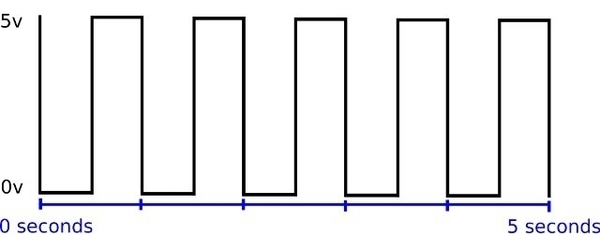
\includegraphics[width=0.7\textwidth]{pwm.jpeg}
    \caption{Een voorbeeld van een PWM signaal}
\end{figure}

\begin{wrapfigure}{r}{0.5\textwidth}
    \centering
    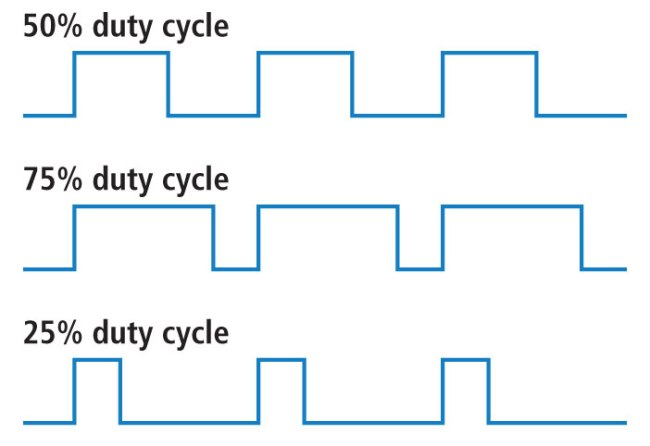
\includegraphics[width=0.48\textwidth]{pwm_duty.jpeg}
    \caption{25\%, 50\%, 75\% PWM signaal voorbeelden}
\end{wrapfigure}
Een andere eigenschap van dit type signaal is de "Duty cycle". Deze wordt in \% gegeven en defineerd hoeveel \% van de tijd het signaal in de HIGH staat is.

We kunnen deze techniek gebruiken om analoge resultaten te krijgen met digitale middelen. Zo kunnen we een PWM signaal gebruik om de helderheid van een LEDje te veranderen ipv het normale aan uit gedrag van digitale pins.\\\\
Met de Arduino kunnen we de \code{analogWrite(pin, x)} functie gebruiken. De \code{analogWrite} functie kan $2^8$ verschillende waarden aannemen, dit wil dus zeggen dat x tussen de 0-255 kan zijn waar 0 correspondeerd met een 0\% duty cycle en 255 met een 100\% duty cycle.

\subsection{Analoge pins}
Analoge pins kunnen enkel als input fungeren. Deze worden gebruikt om bv analoge sensors te lezen. Een analoge sensor die bv aan een analoge pin gekoppeld is zal een spanning leveren op de pin. De Arduino zal deze spanning voor ons vertalen in een numerieke waarde. Daarvoor gebruikt de Arduino een conversie chip, de chip op de Arduino Uno rev3 bezit een chip met een resolutie van 10 bits. Dit wil zeggen dat de pin $2^{10}$ ofwel $1024$ unieke waarden kan aannemen. We kunnen dus waarden van $0-1023$ verwachten. We kunnen de waarde aflezen van de pin met \code{analogRead(pin)}. 1 extra functionaliteit dat de analoge pins hebben is dat ze ook als digitale pins kunnen gebruikt worden.

\chapter{Labo}
\section{Onderzoeksvraag}
Is het goedkoop automatiseren van zuur-base titraties mogelijk, nauwkeurig genoeg en efficiënt?

\section{Meetprincipe}
Zuren en basen splitsen H\textsuperscript{+} en OH\textsuperscript{-} ionen af in waterige oplossing. Deze ionen combineren dan terug om H\textsubscript{2}O te vormen. De concentratie van H\textsuperscript{+} of OH\textsuperscript{-} zal de pH van de oplossing beïnvloeden. De pH van een oplossing kunnen we meten en dus ook een titratiecurve opstellen. Met de titratiecurve kunnen we het equivalentiepunt bepalen. Het equivalentiepunt kunnen we dan gebruiken om de onbekende concentratie te bepalen want $c_1V_1 = c_2V_2$.

\section{Benodigdheden}
\begin{itemize}
    \item pH-meter
    \item 0.1 molair NaOH, HCl, H\textsubscript{2}SO\textsubscript{4}
    \item Fenolftaleïne
    \item Gummidarmpjes
    \item Arduino
    \item Peristaltische pomp en pH circuit
    \item Windows pc
\end{itemize}

\newpage

\section{Werkwijze en opstelling}
Opstelling:
\begin{figure}[H]
    \centering
    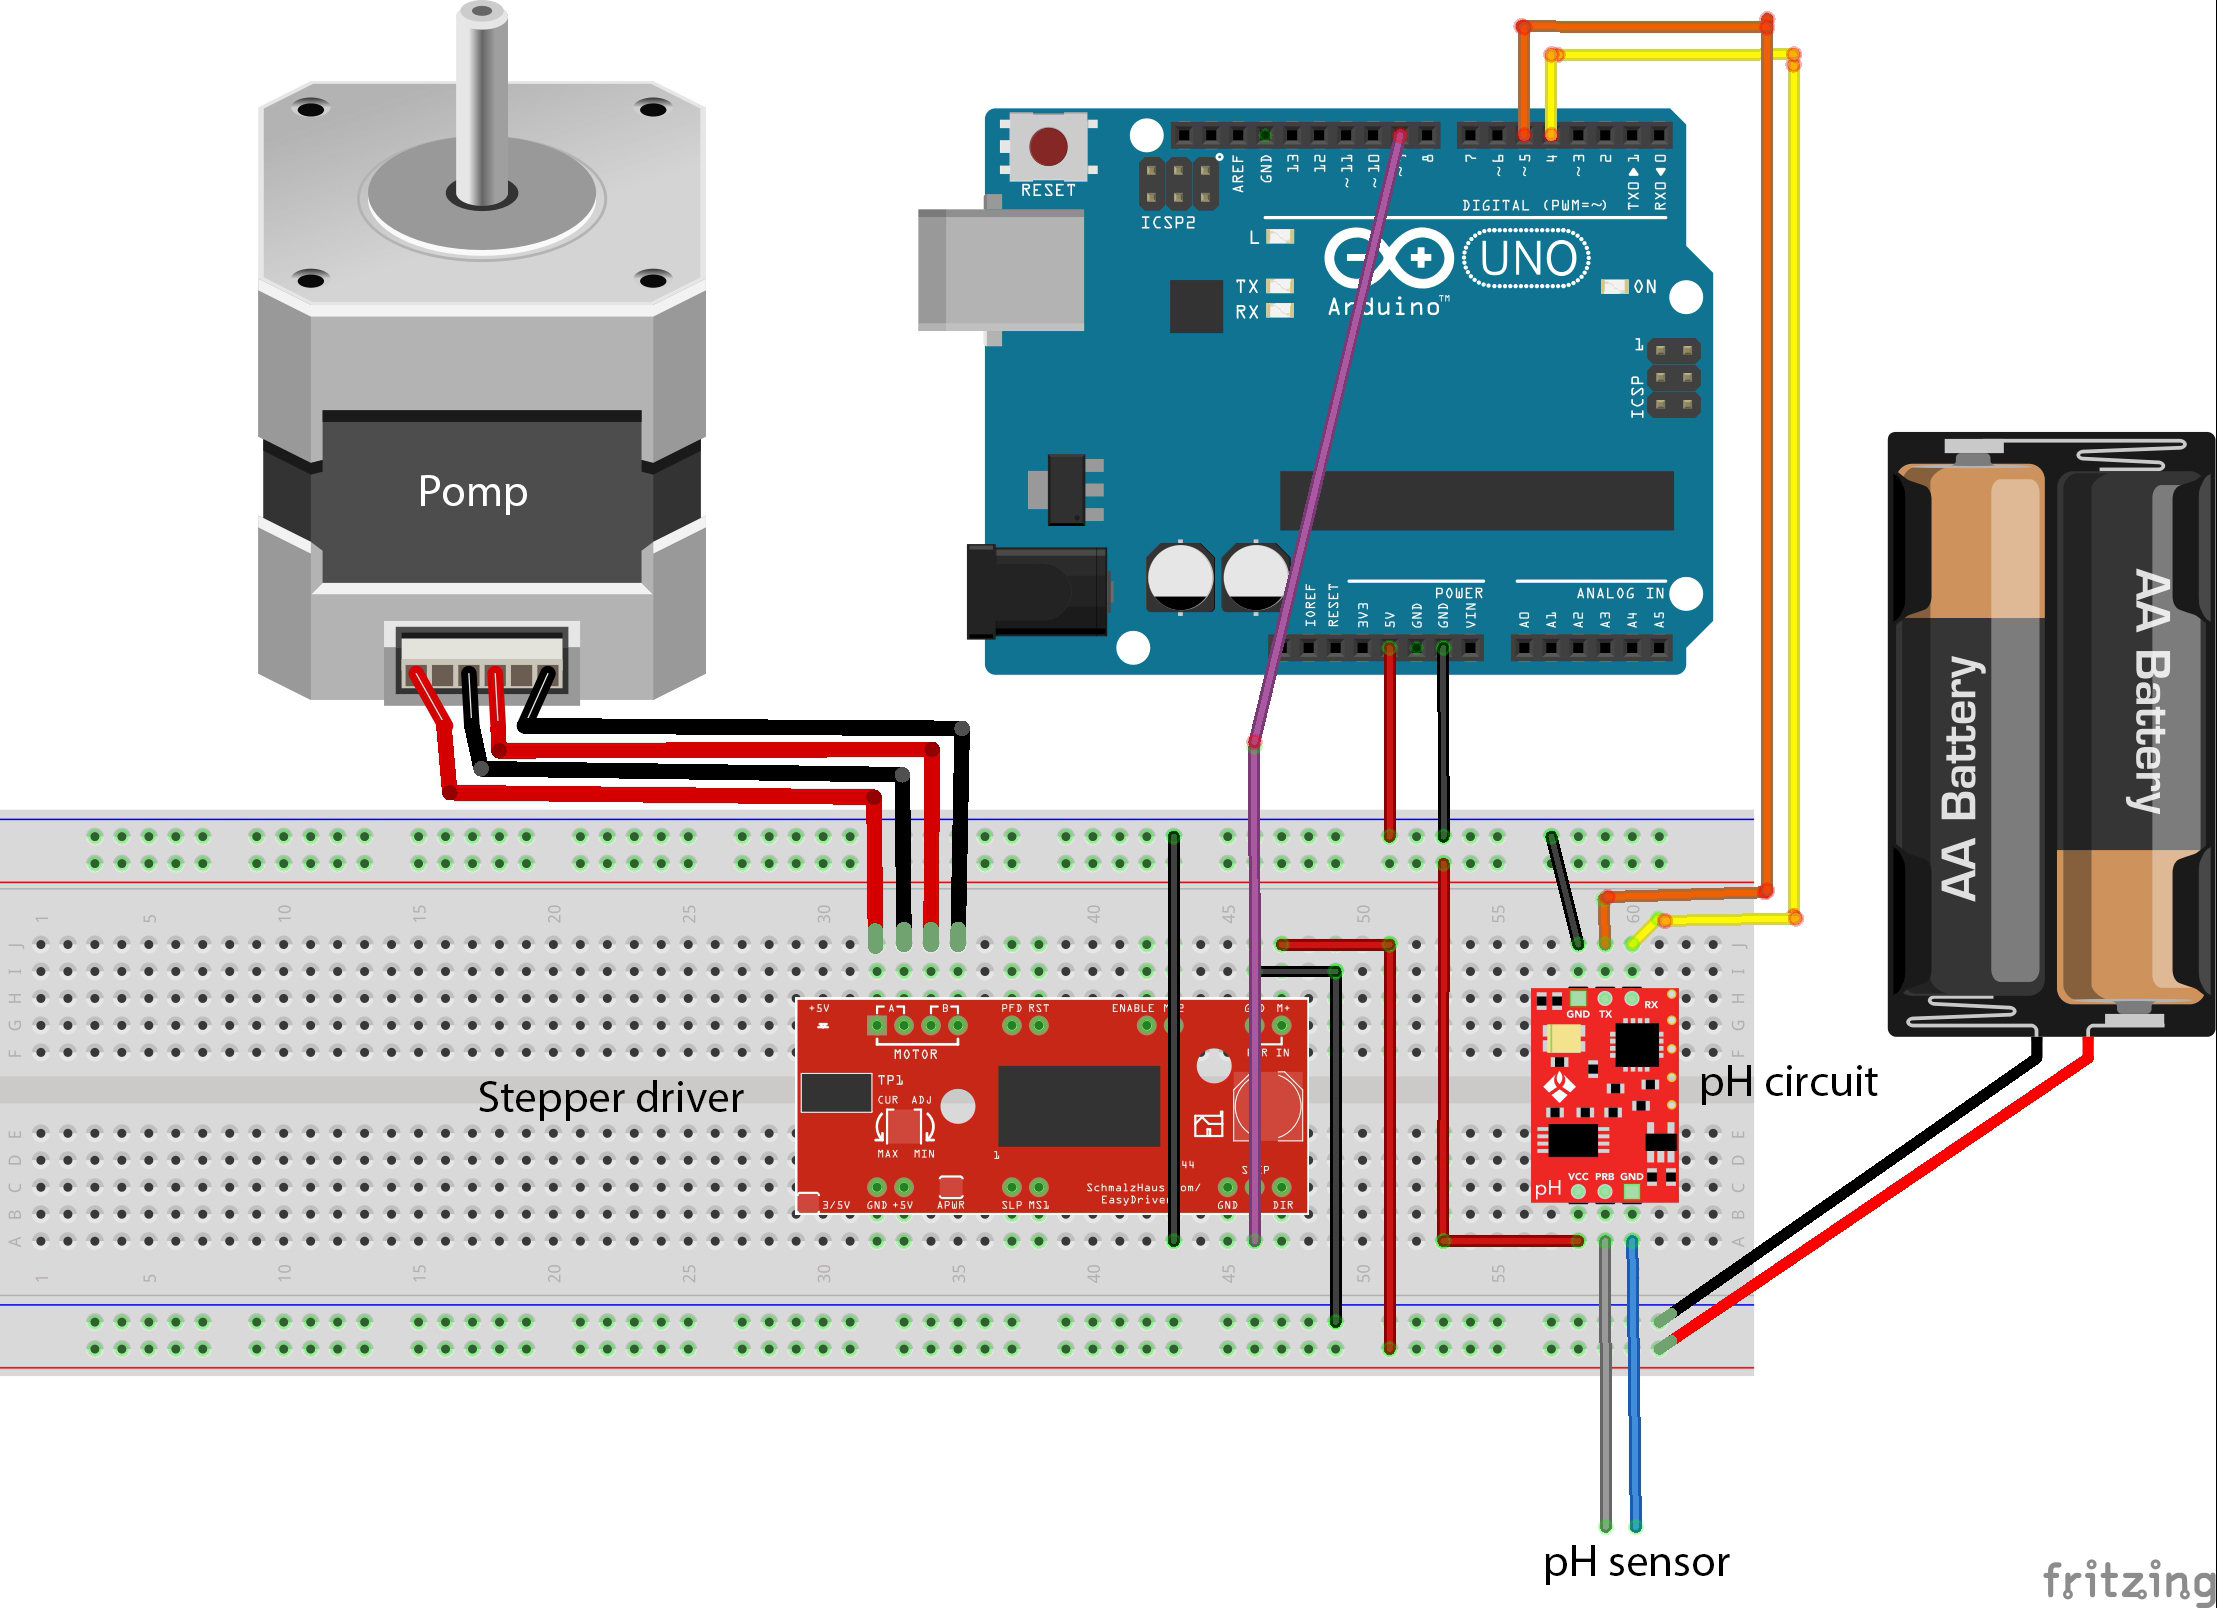
\includegraphics[width=0.9\textwidth]{opstelling.jpg}
    \caption{Arduino circuit opstelling}
\end{figure}
Werkwijze:
\begin{itemize}
    \item Maak 3 oplossingen, HCl, NaOH, H\textsubscript{2}SO\textsubscript{4} elk van 0.1M.
    \item Vul een erlenmyer met 20mL NaOH oplossing + fenolftaleïne.
    \item Vul buret met HCl of H\textsubscript{2}SO\textsubscript{4} oplossing.
    \item Titreer met elke stof 3 maal.
    \item Herhaal maar deze keer gebruikmakende van de arduino opstelling en een pH-sensor ipv fenolftaleïne.
    \item Herhaal nogmaals maar gebruikmakende van een professionele titratiemachine.
\end{itemize}

\newpage

\section{Metingen en analyze}
\subsection{Constanten en formules}
\begin{equation*}
        \text{procentuele mogelijke meetfout} = \frac{\text{onauwkeurigheid}}{\text{gemeten waarde}}*100\%,\ \text{procentuele afwijking} = abs(\frac{x_{exp}}{x_{eig}}*100-100)
\end{equation*}
\begin{tabular}{|c|c|c|c|}
    \hline
                        & HCl & H$_2$SO$_4$ & HSO$_4^-$ \\\hline
    K\textsubscript{a}  & $>1$ & $>1$ & $1.2*10^{-2}$ \\\hline
    pK\textsubscript{a} & $<1$ & $<1$ & $1.92$ \\\hline
\end{tabular}
\quad
\begin{tabular}{|c|c|}
    \hline
        & NaOH \\\hline
    K\textsubscript{b} & $>1$ \\\hline
    pK\textsubscript{b} & $<1$ \\\hline
\end{tabular}

\begin{equation*}
    \begin{split}
        n_1 &= n_2\\
        c_1V_1 &= c_2V_2\\
        c_1 &= \frac{c_2V_2}{V_1}\\
        V_1 &= \frac{c_2V_2}{c_1}\\
    \end{split}
\end{equation*}

\begin{multicols}{2}
\begin{equation*}
    \begin{split}
        A &\xrightleftharpoons[]{H_2O} A^- + H^+\\
        K_a &= \frac{[A^-][H^+]}{[A]}\\
        pKa &= -\log(K_a)\\
    \end{split}
\end{equation*}
\break
\begin{equation*}
    \begin{split}
        B &\xrightleftharpoons[]{H_2O} B^+ + OH^-\\
        K_b &= \frac{[B^+][OH^-]}{[B]}\\
        pK_b &= -\log(K_b)\\
    \end{split}
\end{equation*}
\end{multicols}
Als $K > 1$ dan dissocieert de stof volledig. Gebruikmakende van bovenstaande formules kunnen we het volgende afleiden.\\
\begin{equation*}
    \begin{split}
        &\begin{cases}
            K = \frac{x^2}{y}, & \iff K < 1\\
            n = x + y, & \\
        \end{cases}\\
        &\Longrightarrow\\
        &\begin{cases}
            x = \frac{1}{2}(-K + \sqrt{K}\sqrt{K + 4n}), & \iff K < 1 \wedge n \geq 0 \\
            y = \frac{1}{2}(K + 2n - \sqrt{K}\sqrt{K + 4n}), & \iff K < 1 \wedge n \geq 0\\
        \end{cases}\\
    \end{split}
\end{equation*}

\newpage

\subsection{Handmatig}
\subsubsection{Gegevens}
\begin{tabular}{|l|c|c|c||c|c|c|}
    \hline
      & HCl$_a$ & HCl$_b$ & HCl$_c$ & H$_2$SO$_{4_a}$ & H$_2$SO$_{4_b}$ & H$_2$SO$_{4_c}$ \\\hline
    V (mL) & 22.1 & 21.9 & 22.2 & 11.5 & 11.8 & 11.6 \\\hline
\end{tabular}
\subsubsection{Berekeningen}
\begin{multicols}{2}
    HCl:\\
    \begin{equation*}
        \begin{split}
            c_{NaOH} &= \frac{c_2V_2}{V_1}\\
            c_{NaOH,a} &= \frac{0.1\ mol/L\ 0.020\ L}{0.0221\ L}\\
                    &= \bold{0.091\ mol/L}\\\\
            c_{NaOH,b} &= \frac{0.1\ mol/L\ 0.020\ L}{0.0219\ L}\\
                    &= \bold{0.091\ mol/L}\\\\
            c_{NaOH,c} &= \frac{0.1\ mol/L\ 0.020\ L}{0.0222\ L}\\
                    &= \bold{0.090\ mol/L}\\
        \end{split}
    \end{equation*}
\break
    H\textsubscript{2}SO\textsubscript{4}:\\
    \begin{equation*}
        \begin{split}
            n &= cV\\
            n_{HSO_4^-,a} &= 0.1\ mol/L\ 0.0115\ L\\
                &= \bold{0.00115\ mol}\\\\
            n_{HSO_4^-,b} &= 0.1\ mol/L\ 0.0118\ L\\
                &= \bold{0.00118\ mol}\\\\
            n_{HSO_4^-,c} &= 0.1\ mol/L\ 0.0116\ L\\
                &= \bold{0.00116\ mol}\\\\
        \end{split}
    \end{equation*}
\end{multicols}

\begin{equation*}
    \begin{split}
        n_{SO_4^{2-}} &= \frac{1}{2}(-K + \sqrt{K}\sqrt{K + 4n}), & \iff K < 1 \wedge n \geq 0 \\
        n_{SO_4^{2-},a} &= \frac{1}{2}(-1.2*10^{-2} + \sqrt{1.2*10^{-2}}\sqrt{1.2*10^{-2} + 4*0.00105})\\
            &= \bold{0.00106\ mol}\\
        n_{SO_4^{2-},b} &= \frac{1}{2}(-1.2*10^{-2} + \sqrt{1.2*10^{-2}}\sqrt{1.2*10^{-2} + 4*0.00108})\\
            &= \bold{0.00108\ mol}\\
        n_{SO_4^{2-},c} &= \frac{1}{2}(-1.2*10^{-2} + \sqrt{1.2*10^{-2}}\sqrt{1.2*10^{-2} + 4*0.00106})\\
            &= \bold{0.00107\ mol}\\
        c_{NaOH} &= \frac{n}{V_{NaOH}}\\
        c_{NaOH,a}  &= \frac{0.00115\ mol + 0.00106\ mol}{0.020\ L}\\
            &= \bold{0.111\ mol/L}\\
        c_{NaOH,b}  &= \frac{0.00118\ mol + 0.00108\ mol}{0.020\ L}\\
            &= \bold{0.113\ mol/L}\\
        c_{NaOH,c} &= \frac{0.00116\ mol + 0.00107\ mol}{0.020\ L}\\
            &= \bold{0.111\ mol/L}\\
    \end{split}
\end{equation*}

\newpage

\begin{multicols}{2}
    HCl:\\
    \begin{equation*}
        \begin{split}
            PA_a &= abs(\frac{0.091\ mol/L}{0.1\ mol/L}*100-100)\\
                &= \bold{9\%} \\
            PA_b &= abs(\frac{0.091\ mol/L}{0.1\ mol/L}*100-100)\\
                &= \bold{9\%} \\
            PA_c &= abs(\frac{0.090\ mol/L}{0.1\ mol/L}*100-100)\\
                &= \bold{10\%} \\
            PMM_a &= \frac{0.0001\ L}{0.0221\ L}*100\%\\
                &= \bold{4.5\%}\\
            PMM_b &= \frac{0.0001\ L}{0.0219\ L}*100\%\\
                &= \bold{4.6\%}\\
            PMM_c &= \frac{0.001\ L}{0.0222\ L}*100\%\\
                &= \bold{4.5\%}\\
        \end{split}
    \end{equation*}
\break
    H\textsubscript{2}SO\textsubscript{4}:\\
    \begin{equation*}
        \begin{split}
            PA_a &= abs(\frac{0.111\ mol/L}{0.1\ mol/L}*100-100)\\
                &= \bold{11\%} \\
            PA_b &= abs(\frac{0.113\ mol/L}{0.1\ mol/L}*100-100)\\
                &= \bold{13\%} \\
            PA_c &= abs(\frac{0.111\ mol/L}{0.1\ mol/L}*100-100)\\
                &= \bold{11\%} \\
            PMM_a &= \frac{0.0001\ L}{0.0115\ L}*100\%\\
                &= \bold{8.7\%}\\
            PMM_b &= \frac{0.0001\ L}{0.0118\ L}*100\%\\
                &= \bold{8.5\%}\\
            PMM_c &= \frac{0.001\ L}{0.0116\ L}*100\%\\
                &= \bold{8.6\%}\\
        \end{split}
    \end{equation*}
\end{multicols}

\subsubsection{Resultaten}
\begin{tabular}{|l|c|c|c||c|c|c|}
    \hline
      & HCl$_a$ & HCl$_b$ & HCl$_c$ & H$_2$SO$_{4_a}$ & H$_2$SO$_{4_b}$ & H$_2$SO$_{4_c}$ \\\hline
    c (mol/L) & $0.091\pm4.5\%$ & $0.091\pm4.6\%$ & $0.090\pm4.5\%$ & $0.111\pm8.7\%$ & $0.113\pm8.5\%$ & $0.111\pm8.6\%$ \\\hline
    PA        & 9\% & 9\% & 10\% & 11\% & 13\% & 11\% \\\hline
\end{tabular}

\newpage

\subsection{Arduino}
\subsubsection{Gegevens}
\begin{tabular}{|c|c||c|c||c|c|}
    \hline
    $V_{HCl,a}$ (L) & $pH_{HCl,a}$ & $V_{HCl,b}$ (L) & $pH_{HCl,b}$ & $V_{HCl,c}$ (L) & $pH_{HCl,c}$ \\\hline
    .00000 & 11.32 & .00000 & 11.39 & .00000 & 11.20\\\hline
    \vdots & \vdots & \vdots & \vdots & \vdots & \vdots \\\hline
\end{tabular}\\\\
Het equivalentiepunt is waar de titratiecurve een afgeleide heeft van $\pm\infinity$. Hier kunnen we gebruikmaken van Mathematica om onze data als volgt te analyseren.\\\\
Eerst passen we de "Interpolation" functie toe om een best passende curve voor onze gegevensset te vinden.
\begin{figure}[H]
    \centering
    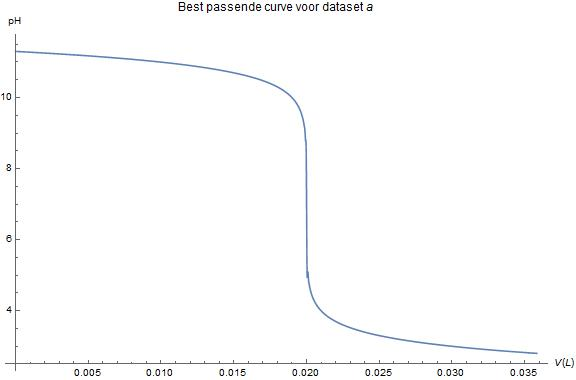
\includegraphics[width=0.7\textwidth]{a_interpolation.jpg}
    \caption{"Interpolation" functie toegepast op dataset a}
\end{figure}
\begin{figure}[H]
    \centering
    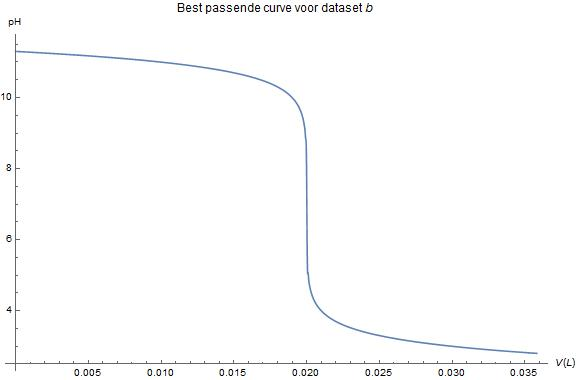
\includegraphics[width=0.7\textwidth]{b_interpolation.jpg}
    \caption{"Interpolation" functie toegepast op dataset b}
\end{figure}
\begin{figure}[H]
    \centering
    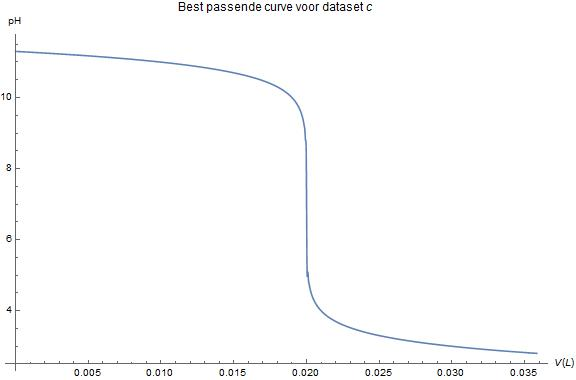
\includegraphics[width=0.7\textwidth]{c_interpolation.jpg}
    \caption{"Interpolation" functie toegepast op dataset c}
\end{figure}
\newpage
Daarna kunnen we de afgeleiden nemen van deze functies met de "Derivative" functie.\\
\begin{figure}[H]
    \centering
    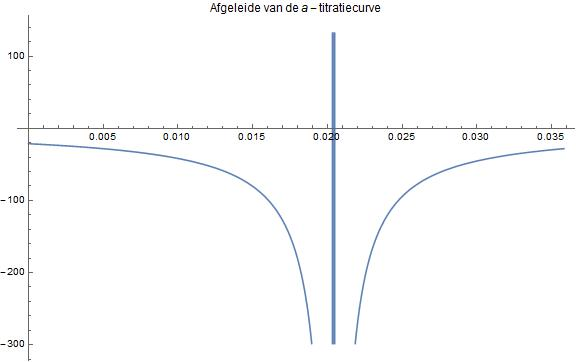
\includegraphics[width=0.7\textwidth]{a_derivative.jpg}
    \caption{"Derivative" functie toegepast op a-titratiecurve}
\end{figure}
\begin{figure}[H]
    \centering
    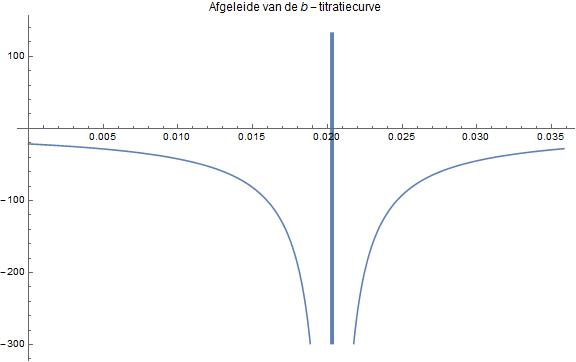
\includegraphics[width=0.7\textwidth]{b_derivative.jpg}
    \caption{"Derivative" functie toegepast op b-titratiecurve}
\end{figure}
\begin{figure}[H]
    \centering
    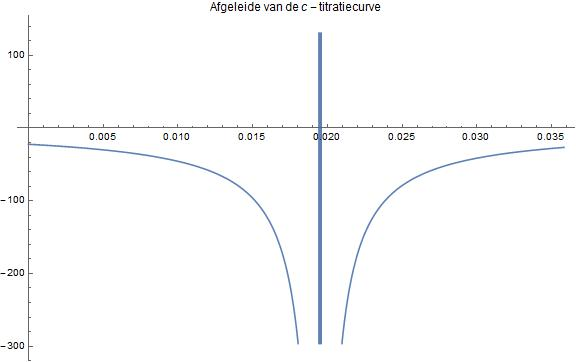
\includegraphics[width=0.7\textwidth]{c_derivative.jpg}
    \caption{"Derivative" functie toegepast op c-titratiecurve}
\end{figure}
Hiervan nemen we dan de x-waarde van het minima en dat is ons volume.\\\\
\begin{tabular}{|c|c|c|}
    \hline
    $V_{a}$ (L) & $V_{b}$ (L) & $V_{c}$ (L) \\\hline
    0.0204 & 0.0205 & 0.0194 \\\hline
\end{tabular}

\begin{equation*}
    \begin{split}
        c_{NaOH} &= \frac{0.1\ mol/L * 0.020\ L}{V}\\
        c_{NaOH,a} &= \frac{0.1\ mol/L * 0.020\ L}{0.0204\ L}\\
            &= \bold{0.098\ mol\ L}\\\\
        c_{NaOH,b} &= \frac{0.1\ mol/L * 0.020\ L}{0.0205\ L}\\
            &= \bold{0.098\ mol\ L}\\\\
        c_{NaOH,c} &= \frac{0.1\ mol/L * 0.020\ L}{0.0194\ L}\\
            &= \bold{0.103\ mol\ L}\\
    \end{split}
\end{equation*}

\begin{multicols}{2}
    \begin{equation*}
        \begin{split}
            PA_a &= abs(\frac{0.098\ mol/L}{0.1\ mol/L}*100-100)\\
                &= \bold{2\%} \\
            PA_b &= abs(\frac{0.098\ mol/L}{0.1\ mol/L}*100-100)\\
                &= \bold{2\%} \\
            PA_c &= abs(\frac{0.103\ mol/L}{0.1\ mol/L}*100-100)\\
                &= \bold{3\%} \\
        \end{split}
    \end{equation*}
\break
    \begin{equation*}
        \begin{split}
            PMM_a &= \frac{0.0001\ L}{0.0204\ L}*100\%\\
                &= \bold{4.9\%}\\
            PMM_b &= \frac{0.0001\ L}{0.0205\ L}*100\%\\
                &= \bold{4.9\%}\\
            PMM_c &= \frac{0.001\ L}{0.0194\ L}*100\%\\
                &= \bold{5.2\%}\\
        \end{split}
    \end{equation*}
\end{multicols}

\subsubsection{Resultaten}
\begin{tabular}{|c|c|c|c|}
    \hline
    & HCL\textsubscript{a} & HCl\textsubscript{b} & HCl\textsubscript{c} \\\hline
    c (mol/L) & 0.098$\pm$4.9\% & 0.098$\pm$4.9\% & 0.103$\pm$5.2\% \\\hline
    PA  & 2\% & 2\% & 3\% \\\hline
\end{tabular}

\newpage

\subsection{Professionele machine}
Moet nog uitgevoerd worden.

\section{Besluiten}

\section{Reflectie}
\begin{itemize}
    \item De uitvoering met Arduino verliep iets moeilijker omdat Arduino nog niet volledig klaar was.
    \item Het effectieve labo was makkelijk uit te voeren maar heb titratie van H\textsubscript{2}SO\textsubscript{4} met NaOH niet kunnen uitvoeren mits tijdsgebrek. Ik had het gedeelte met H\textsubscript{2}SO\textsubscript{4} vooraf niet gepland maar tijdens het labo zag ik dat ik nog tijd over had en probeerde die tijd dan ook te gebruiken maar heb het alleen maar manueel kunnen uitvoeren.
\end{itemize}

\printbibliography

\begin{appendices}
\chapter{Data}
\begin{longtable}{|c|c||c|c||c|c|}
    \hline
    $V_{HCl,a}$ (L) & $pH_{HCl,a}$ & $V_{HCl,b}$ (L) & $pH_{HCl,b}$ & $V_{HCl,c}$ (L) & $pH_{HCl,c}$ \\\hline
.00000 & 11.32 & .00000 & 11.39 & .00000 & 11.20\\\hline
.00005 & 11.30 & .00004 & 11.30 & .00005 & 11.36\\\hline
.00011 & 11.30 & .00009 & 11.31 & .00009 & 11.25\\\hline
.00015 & 11.35 & .00013 & 11.30 & .00014 & 11.35\\\hline
.00021 & 11.25 & .00019 & 11.24 & .00019 & 11.23\\\hline
.00025 & 11.30 & .00023 & 11.37 & .00025 & 11.31\\\hline
.00031 & 11.29 & .00027 & 11.35 & .00031 & 11.34\\\hline
.00035 & 11.21 & .00032 & 11.35 & .00036 & 11.29\\\hline
.00040 & 11.29 & .00036 & 11.32 & .00040 & 11.25\\\hline
.00044 & 11.23 & .00041 & 11.38 & .00046 & 11.29\\\hline
.00048 & 11.31 & .00046 & 11.35 & .00050 & 11.29\\\hline
.00052 & 11.29 & .00052 & 11.28 & .00056 & 11.29\\\hline
.00056 & 11.29 & .00058 & 11.29 & .00060 & 11.25\\\hline
.00062 & 11.19 & .00064 & 11.30 & .00065 & 11.37\\\hline
.00066 & 11.24 & .00069 & 11.20 & .00070 & 11.29\\\hline
.00071 & 11.34 & .00073 & 11.28 & .00075 & 11.25\\\hline
.00077 & 11.37 & .00077 & 11.28 & .00080 & 11.36\\\hline
.00083 & 11.28 & .00082 & 11.28 & .00085 & 11.31\\\hline
.00087 & 11.37 & .00087 & 11.28 & .00089 & 11.28\\\hline
.00093 & 11.27 & .00092 & 11.21 & .00093 & 11.28\\\hline
.00099 & 11.23 & .00096 & 11.23 & .00098 & 11.28\\\hline
.00103 & 11.28 & .00101 & 11.28 & .00103 & 11.24\\\hline
.00107 & 11.20 & .00106 & 11.27 & .00107 & 11.31\\\hline
.00113 & 11.30 & .00112 & 11.33 & .00112 & 11.28\\\hline
.00118 & 11.27 & .00118 & 11.27 & .00117 & 11.29\\\hline
.00123 & 11.26 & .00123 & 11.21 & .00123 & 11.19\\\hline
.00129 & 11.27 & .00127 & 11.28 & .00129 & 11.27\\\hline
.00134 & 11.20 & .00132 & 11.28 & .00134 & 11.31\\\hline
.00139 & 11.27 & .00137 & 11.27 & .00140 & 11.34\\\hline
.00143 & 11.27 & .00141 & 11.27 & .00146 & 11.24\\\hline
.00147 & 11.19 & .00146 & 11.27 & .00152 & 11.35\\\hline
.00151 & 11.27 & .00151 & 11.27 & .00158 & 11.27\\\hline
.00157 & 11.22 & .00157 & 11.27 & .00163 & 11.26\\\hline
.00161 & 11.26 & .00162 & 11.36 & .00169 & 11.25\\\hline
.00165 & 11.26 & .00166 & 11.26 & .00174 & 11.25\\\hline
.00169 & 11.25 & .00172 & 11.26 & .00180 & 11.32\\\hline
.00174 & 11.31 & .00177 & 11.36 & .00186 & 11.26\\\hline
.00180 & 11.19 & .00181 & 11.26 & .00191 & 11.19\\\hline
.00186 & 11.26 & .00185 & 11.28 & .00197 & 11.26\\\hline
.00192 & 11.26 & .00189 & 11.20 & .00202 & 11.23\\\hline
.00197 & 11.26 & .00195 & 11.26 & .00206 & 11.25\\\hline
.00201 & 11.26 & .00200 & 11.22 & .00211 & 11.34\\\hline
.00206 & 11.23 & .00204 & 11.17 & .00215 & 11.25\\\hline
.00210 & 11.19 & .00208 & 11.28 & .00220 & 11.24\\\hline
.00216 & 11.31 & .00213 & 11.33 & .00226 & 11.27\\\hline
.00220 & 11.33 & .00218 & 11.25 & .00232 & 11.25\\\hline
.00225 & 11.28 & .00222 & 11.16 & .00237 & 11.32\\\hline
.00229 & 11.25 & .00227 & 11.21 & .00242 & 11.25\\\hline
.00233 & 11.25 & .00232 & 11.27 & .00246 & 11.24\\\hline
.00239 & 11.19 & .00238 & 11.25 & .00251 & 11.31\\\hline
.00243 & 11.19 & .00243 & 11.24 & .00255 & 11.24\\\hline
.00249 & 11.24 & .00248 & 11.20 & .00260 & 11.28\\\hline
.00253 & 11.21 & .00254 & 11.22 & .00266 & 11.24\\\hline
.00258 & 11.29 & .00258 & 11.21 & .00270 & 11.21\\\hline
.00263 & 11.25 & .00262 & 11.21 & .00274 & 11.29\\\hline
.00269 & 11.24 & .00266 & 11.33 & .00280 & 11.19\\\hline
.00274 & 11.27 & .00271 & 11.24 & .00285 & 11.23\\\hline
.00280 & 11.31 & .00277 & 11.15 & .00290 & 11.33\\\hline
.00284 & 11.22 & .00281 & 11.23 & .00295 & 11.17\\\hline
.00288 & 11.22 & .00285 & 11.23 & .00300 & 11.32\\\hline
.00292 & 11.23 & .00290 & 11.23 & .00306 & 11.23\\\hline
.00298 & 11.18 & .00296 & 11.23 & .00310 & 11.28\\\hline
.00303 & 11.23 & .00300 & 11.23 & .00316 & 11.32\\\hline
.00307 & 11.23 & .00304 & 11.18 & .00320 & 11.14\\\hline
.00313 & 11.23 & .00310 & 11.16 & .00324 & 11.26\\\hline
.00318 & 11.23 & .00316 & 11.28 & .00328 & 11.23\\\hline
.00324 & 11.27 & .00321 & 11.22 & .00333 & 11.22\\\hline
.00330 & 11.20 & .00326 & 11.24 & .00337 & 11.22\\\hline
.00336 & 11.22 & .00332 & 11.14 & .00341 & 11.23\\\hline
.00342 & 11.22 & .00338 & 11.18 & .00345 & 11.30\\\hline
.00346 & 11.26 & .00343 & 11.26 & .00349 & 11.31\\\hline
.00352 & 11.13 & .00349 & 11.25 & .00354 & 11.29\\\hline
.00356 & 11.22 & .00355 & 11.22 & .00360 & 11.17\\\hline
.00360 & 11.16 & .00360 & 11.24 & .00366 & 11.30\\\hline
.00365 & 11.29 & .00364 & 11.21 & .00372 & 11.20\\\hline
.00369 & 11.22 & .00369 & 11.29 & .00378 & 11.17\\\hline
.00373 & 11.28 & .00373 & 11.12 & .00383 & 11.21\\\hline
.00377 & 11.31 & .00377 & 11.23 & .00389 & 11.17\\\hline
.00381 & 11.13 & .00383 & 11.29 & .00393 & 11.21\\\hline
.00386 & 11.21 & .00389 & 11.13 & .00397 & 11.29\\\hline
.00391 & 11.21 & .00395 & 11.26 & .00403 & 11.20\\\hline
.00395 & 11.21 & .00399 & 11.20 & .00407 & 11.14\\\hline
.00399 & 11.19 & .00403 & 11.20 & .00411 & 11.20\\\hline
.00405 & 11.20 & .00409 & 11.20 & .00416 & 11.20\\\hline
.00411 & 11.11 & .00415 & 11.18 & .00421 & 11.23\\\hline
.00417 & 11.10 & .00420 & 11.20 & .00425 & 11.25\\\hline
.00421 & 11.27 & .00425 & 11.16 & .00430 & 11.29\\\hline
.00425 & 11.21 & .00431 & 11.20 & .00436 & 11.22\\\hline
.00431 & 11.20 & .00437 & 11.25 & .00440 & 11.26\\\hline
.00437 & 11.19 & .00441 & 11.19 & .00446 & 11.25\\\hline
.00441 & 11.09 & .00445 & 11.26 & .00451 & 11.17\\\hline
.00446 & 11.18 & .00450 & 11.21 & .00456 & 11.17\\\hline
.00450 & 11.19 & .00455 & 11.15 & .00460 & 11.20\\\hline
.00454 & 11.19 & .00461 & 11.22 & .00465 & 11.19\\\hline
.00460 & 11.27 & .00465 & 11.19 & .00471 & 11.27\\\hline
.00465 & 11.26 & .00469 & 11.10 & .00477 & 11.18\\\hline
.00471 & 11.12 & .00474 & 11.22 & .00483 & 11.28\\\hline
.00475 & 11.14 & .00478 & 11.19 & .00489 & 11.18\\\hline
.00481 & 11.16 & .00483 & 11.18 & .00493 & 11.15\\\hline
.00487 & 11.20 & .00488 & 11.16 & .00498 & 11.12\\\hline
.00492 & 11.10 & .00493 & 11.08 & .00503 & 11.11\\\hline
.00496 & 11.18 & .00497 & 11.18 & .00507 & 11.18\\\hline
.00501 & 11.19 & .00503 & 11.08 & .00511 & 11.16\\\hline
.00506 & 11.17 & .00508 & 11.10 & .00517 & 11.17\\\hline
.00510 & 11.22 & .00512 & 11.17 & .00523 & 11.22\\\hline
.00515 & 11.09 & .00517 & 11.18 & .00529 & 11.17\\\hline
.00519 & 11.12 & .00523 & 11.17 & .00533 & 11.21\\\hline
.00523 & 11.07 & .00527 & 11.25 & .00539 & 11.18\\\hline
.00529 & 11.25 & .00531 & 11.17 & .00544 & 11.16\\\hline
.00535 & 11.17 & .00537 & 11.07 & .00550 & 11.16\\\hline
.00540 & 11.16 & .00542 & 11.11 & .00554 & 11.16\\\hline
.00546 & 11.19 & .00548 & 11.07 & .00560 & 11.19\\\hline
.00552 & 11.25 & .00553 & 11.16 & .00566 & 11.16\\\hline
.00558 & 11.14 & .00557 & 11.18 & .00570 & 11.16\\\hline
.00563 & 11.13 & .00561 & 11.13 & .00575 & 11.09\\\hline
.00567 & 11.16 & .00566 & 11.11 & .00580 & 11.15\\\hline
.00573 & 11.15 & .00572 & 11.11 & .00584 & 11.11\\\hline
.00578 & 11.08 & .00577 & 11.15 & .00589 & 11.15\\\hline
.00582 & 11.10 & .00581 & 11.13 & .00593 & 11.22\\\hline
.00588 & 11.06 & .00586 & 11.24 & .00599 & 11.10\\\hline
.00592 & 11.23 & .00591 & 11.15 & .00605 & 11.06\\\hline
.00597 & 11.15 & .00597 & 11.23 & .00609 & 11.15\\\hline
.00603 & 11.21 & .00603 & 11.18 & .00613 & 11.14\\\hline
.00607 & 11.16 & .00609 & 11.14 & .00619 & 11.11\\\hline
.00611 & 11.14 & .00614 & 11.06 & .00625 & 11.04\\\hline
.00617 & 11.18 & .00619 & 11.22 & .00629 & 11.04\\\hline
.00623 & 11.22 & .00624 & 11.14 & .00635 & 11.14\\\hline
.00627 & 11.11 & .00628 & 11.22 & .00639 & 11.13\\\hline
.00633 & 11.15 & .00633 & 11.14 & .00643 & 11.13\\\hline
.00638 & 11.17 & .00639 & 11.13 & .00647 & 11.06\\\hline
.00644 & 11.04 & .00644 & 11.13 & .00653 & 11.15\\\hline
.00648 & 11.13 & .00650 & 11.18 & .00657 & 11.20\\\hline
.00654 & 11.10 & .00655 & 11.13 & .00663 & 11.22\\\hline
.00659 & 11.04 & .00660 & 11.21 & .00668 & 11.21\\\hline
.00665 & 11.05 & .00665 & 11.08 & .00674 & 11.15\\\hline
.00669 & 11.05 & .00670 & 11.12 & .00679 & 11.12\\\hline
.00673 & 11.12 & .00674 & 11.20 & .00684 & 11.12\\\hline
.00678 & 11.19 & .00680 & 11.19 & .00689 & 11.15\\\hline
.00683 & 11.12 & .00684 & 11.05 & .00694 & 11.10\\\hline
.00689 & 11.12 & .00689 & 11.12 & .00699 & 11.15\\\hline
.00695 & 11.02 & .00695 & 11.12 & .00703 & 11.04\\\hline
.00701 & 11.11 & .00699 & 11.11 & .00707 & 11.10\\\hline
.00706 & 11.17 & .00704 & 11.12 & .00711 & 11.11\\\hline
.00711 & 11.11 & .00709 & 11.11 & .00715 & 11.11\\\hline
.00717 & 11.11 & .00714 & 11.05 & .00720 & 11.11\\\hline
.00723 & 11.11 & .00719 & 11.19 & .00724 & 11.06\\\hline
.00728 & 11.15 & .00723 & 11.01 & .00728 & 11.10\\\hline
.00734 & 11.10 & .00727 & 11.09 & .00732 & 11.09\\\hline
.00739 & 11.10 & .00731 & 11.06 & .00737 & 11.10\\\hline
.00745 & 11.00 & .00737 & 11.02 & .00743 & 11.05\\\hline
.00751 & 11.05 & .00741 & 11.17 & .00749 & 11.12\\\hline
.00756 & 11.09 & .00745 & 11.10 & .00754 & 11.10\\\hline
.00762 & 11.09 & .00751 & 11.10 & .00760 & 11.06\\\hline
.00768 & 11.00 & .00756 & 11.01 & .00765 & 11.09\\\hline
.00774 & 11.09 & .00762 & 11.18 & .00770 & 11.13\\\hline
.00780 & 11.09 & .00766 & 11.09 & .00775 & 11.09\\\hline
.00784 & 11.08 & .00770 & 11.09 & .00779 & 11.09\\\hline
.00790 & 11.16 & .00775 & 11.09 & .00783 & 11.14\\\hline
.00796 & 11.06 & .00779 & 11.03 & .00788 & 10.99\\\hline
.00802 & 11.16 & .00784 & 11.04 & .00792 & 11.08\\\hline
.00808 & 11.15 & .00789 & 11.17 & .00798 & 11.11\\\hline
.00812 & 11.06 & .00794 & 10.99 & .00803 & 11.08\\\hline
.00816 & 11.07 & .00799 & 11.01 & .00808 & 10.98\\\hline
.00820 & 11.16 & .00803 & 11.08 & .00814 & 11.11\\\hline
.00824 & 11.07 & .00807 & 11.15 & .00819 & 11.12\\\hline
.00829 & 10.99 & .00812 & 11.07 & .00825 & 11.15\\\hline
.00833 & 11.07 & .00817 & 11.06 & .00831 & 11.16\\\hline
.00839 & 11.12 & .00822 & 11.11 & .00837 & 11.08\\\hline
.00845 & 11.06 & .00827 & 11.14 & .00843 & 11.15\\\hline
.00851 & 11.10 & .00831 & 11.08 & .00848 & 11.06\\\hline
.00856 & 10.99 & .00835 & 11.07 & .00852 & 11.16\\\hline
.00861 & 10.98 & .00839 & 11.06 & .00857 & 11.15\\\hline
.00865 & 11.05 & .00845 & 11.06 & .00861 & 10.98\\\hline
.00869 & 11.06 & .00849 & 11.06 & .00866 & 11.09\\\hline
.00874 & 11.05 & .00855 & 11.04 & .00870 & 11.12\\\hline
.00879 & 11.00 & .00861 & 11.05 & .00875 & 11.05\\\hline
.00883 & 11.05 & .00866 & 11.01 & .00880 & 11.05\\\hline
.00889 & 11.04 & .00870 & 11.05 & .00884 & 11.14\\\hline
.00893 & 11.04 & .00874 & 11.05 & .00890 & 11.02\\\hline
.00897 & 11.07 & .00878 & 11.01 & .00895 & 11.01\\\hline
.00901 & 11.01 & .00882 & 11.05 & .00899 & 11.04\\\hline
.00905 & 10.99 & .00886 & 11.07 & .00904 & 11.04\\\hline
.00911 & 11.04 & .00892 & 11.13 & .00910 & 11.05\\\hline
.00916 & 10.97 & .00896 & 11.07 & .00916 & 11.05\\\hline
.00922 & 11.11 & .00902 & 11.04 & .00922 & 11.10\\\hline
.00928 & 11.03 & .00907 & 11.13 & .00927 & 10.96\\\hline
.00934 & 11.03 & .00913 & 11.00 & .00932 & 11.03\\\hline
.00939 & 11.07 & .00917 & 11.03 & .00938 & 11.03\\\hline
.00944 & 11.03 & .00922 & 11.03 & .00942 & 11.04\\\hline
.00949 & 10.97 & .00928 & 10.96 & .00947 & 11.02\\\hline
.00955 & 11.02 & .00934 & 11.02 & .00952 & 10.96\\\hline
.00959 & 10.96 & .00938 & 10.98 & .00957 & 11.02\\\hline
.00964 & 11.02 & .00942 & 11.02 & .00963 & 11.00\\\hline
.00969 & 11.03 & .00946 & 11.02 & .00968 & 11.01\\\hline
.00974 & 11.01 & .00951 & 11.12 & .00972 & 11.00\\\hline
.00980 & 11.02 & .00957 & 11.02 & .00976 & 11.10\\\hline
.00985 & 11.01 & .00963 & 11.10 & .00981 & 10.95\\\hline
.00990 & 11.00 & .00968 & 11.03 & .00985 & 11.01\\\hline
.00996 & 11.00 & .00972 & 11.01 & .00990 & 11.06\\\hline
.01000 & 11.05 & .00976 & 11.01 & .00996 & 10.92\\\hline
.01004 & 11.00 & .00982 & 11.08 & .01002 & 11.00\\\hline
.01009 & 10.98 & .00986 & 11.02 & .01008 & 11.01\\\hline
.01015 & 10.91 & .00992 & 11.00 & .01013 & 10.99\\\hline
.01019 & 11.08 & .00997 & 10.94 & .01017 & 10.91\\\hline
.01025 & 10.99 & .01001 & 11.00 & .01023 & 11.06\\\hline
.01030 & 10.95 & .01005 & 10.91 & .01027 & 11.04\\\hline
.01034 & 10.98 & .01010 & 11.00 & .01033 & 10.99\\\hline
.01038 & 10.98 & .01015 & 10.99 & .01037 & 10.97\\\hline
.01042 & 11.03 & .01020 & 10.99 & .01041 & 10.98\\\hline
.01046 & 10.98 & .01026 & 10.95 & .01046 & 10.95\\\hline
.01052 & 10.97 & .01031 & 10.97 & .01052 & 10.98\\\hline
.01057 & 10.91 & .01035 & 10.96 & .01056 & 10.98\\\hline
.01061 & 10.89 & .01040 & 11.03 & .01060 & 10.90\\\hline
.01067 & 10.97 & .01045 & 10.98 & .01064 & 10.97\\\hline
.01071 & 10.97 & .01050 & 10.90 & .01070 & 11.05\\\hline
.01077 & 10.97 & .01054 & 11.05 & .01075 & 10.97\\\hline
.01081 & 10.96 & .01059 & 10.97 & .01080 & 10.96\\\hline
.01087 & 10.91 & .01063 & 10.97 & .01084 & 10.99\\\hline
.01093 & 10.89 & .01067 & 11.00 & .01089 & 10.96\\\hline
.01099 & 10.86 & .01071 & 10.97 & .01095 & 10.96\\\hline
.01103 & 10.91 & .01075 & 10.96 & .01101 & 10.88\\\hline
.01108 & 11.03 & .01079 & 10.96 & .01106 & 10.98\\\hline
.01114 & 10.99 & .01085 & 11.03 & .01110 & 10.95\\\hline
.01120 & 11.03 & .01091 & 10.96 & .01116 & 10.94\\\hline
.01126 & 10.96 & .01095 & 11.03 & .01121 & 10.94\\\hline
.01130 & 10.94 & .01099 & 10.97 & .01126 & 11.01\\\hline
.01136 & 10.91 & .01103 & 10.96 & .01132 & 10.89\\\hline
.01140 & 11.02 & .01108 & 10.89 & .01138 & 10.84\\\hline
.01146 & 10.93 & .01113 & 10.91 & .01144 & 10.93\\\hline
.01150 & 10.93 & .01117 & 10.95 & .01150 & 10.93\\\hline
.01156 & 10.93 & .01123 & 11.04 & .01154 & 10.85\\\hline
.01161 & 10.89 & .01127 & 10.94 & .01159 & 10.89\\\hline
.01165 & 11.02 & .01133 & 10.94 & .01165 & 10.96\\\hline
.01170 & 10.96 & .01137 & 10.87 & .01170 & 10.92\\\hline
.01174 & 10.99 & .01141 & 10.96 & .01175 & 10.96\\\hline
.01179 & 10.91 & .01146 & 10.90 & .01179 & 10.91\\\hline
.01184 & 10.91 & .01150 & 11.01 & .01184 & 10.91\\\hline
.01190 & 10.91 & .01154 & 11.02 & .01190 & 11.00\\\hline
.01194 & 10.82 & .01160 & 11.00 & .01194 & 10.91\\\hline
.01200 & 10.90 & .01166 & 10.89 & .01200 & 10.98\\\hline
.01206 & 10.83 & .01171 & 10.92 & .01206 & 10.90\\\hline
.01212 & 10.85 & .01175 & 10.90 & .01210 & 10.90\\\hline
.01216 & 10.82 & .01180 & 11.00 & .01216 & 10.98\\\hline
.01222 & 10.89 & .01184 & 10.95 & .01220 & 10.94\\\hline
.01226 & 10.89 & .01189 & 10.91 & .01224 & 10.83\\\hline
.01231 & 10.89 & .01195 & 10.96 & .01230 & 10.97\\\hline
.01235 & 10.82 & .01199 & 10.82 & .01235 & 10.88\\\hline
.01240 & 10.88 & .01205 & 10.84 & .01240 & 10.81\\\hline
.01244 & 10.86 & .01210 & 10.85 & .01245 & 10.94\\\hline
.01248 & 10.88 & .01215 & 10.85 & .01249 & 10.92\\\hline
.01253 & 10.87 & .01220 & 10.89 & .01254 & 10.87\\\hline
.01257 & 10.92 & .01224 & 10.89 & .01259 & 10.87\\\hline
.01261 & 10.93 & .01228 & 10.91 & .01264 & 10.89\\\hline
.01265 & 10.86 & .01233 & 10.93 & .01270 & 10.86\\\hline
.01269 & 10.86 & .01239 & 10.88 & .01275 & 10.82\\\hline
.01275 & 10.84 & .01245 & 10.91 & .01281 & 10.78\\\hline
.01279 & 10.86 & .01250 & 10.91 & .01286 & 10.85\\\hline
.01283 & 10.76 & .01256 & 10.87 & .01290 & 10.85\\\hline
.01289 & 10.88 & .01260 & 10.87 & .01294 & 10.93\\\hline
.01294 & 10.94 & .01264 & 10.89 & .01300 & 10.76\\\hline
.01298 & 10.92 & .01268 & 10.86 & .01306 & 10.84\\\hline
.01303 & 10.84 & .01274 & 10.94 & .01310 & 10.84\\\hline
.01308 & 10.85 & .01279 & 10.86 & .01316 & 10.84\\\hline
.01312 & 10.84 & .01285 & 10.95 & .01320 & 10.76\\\hline
.01317 & 10.83 & .01289 & 10.75 & .01324 & 10.83\\\hline
.01321 & 10.79 & .01294 & 10.87 & .01328 & 10.77\\\hline
.01325 & 10.79 & .01299 & 10.92 & .01332 & 10.77\\\hline
.01331 & 10.79 & .01304 & 10.79 & .01336 & 10.82\\\hline
.01335 & 10.74 & .01308 & 10.84 & .01342 & 10.77\\\hline
.01341 & 10.89 & .01313 & 10.76 & .01348 & 10.81\\\hline
.01346 & 10.82 & .01319 & 10.89 & .01352 & 10.80\\\hline
.01350 & 10.90 & .01325 & 10.83 & .01358 & 10.73\\\hline
.01355 & 10.85 & .01330 & 10.83 & .01362 & 10.80\\\hline
.01361 & 10.77 & .01334 & 10.81 & .01367 & 10.71\\\hline
.01366 & 10.81 & .01340 & 10.86 & .01372 & 10.80\\\hline
.01370 & 10.81 & .01345 & 10.79 & .01376 & 10.82\\\hline
.01375 & 10.76 & .01349 & 10.88 & .01380 & 10.89\\\hline
.01381 & 10.79 & .01353 & 10.81 & .01384 & 10.72\\\hline
.01386 & 10.77 & .01357 & 10.77 & .01390 & 10.85\\\hline
.01392 & 10.87 & .01362 & 10.80 & .01396 & 10.74\\\hline
.01396 & 10.84 & .01367 & 10.74 & .01401 & 10.85\\\hline
.01400 & 10.73 & .01373 & 10.80 & .01406 & 10.77\\\hline
.01406 & 10.74 & .01379 & 10.79 & .01412 & 10.70\\\hline
.01412 & 10.68 & .01383 & 10.85 & .01416 & 10.77\\\hline
.01416 & 10.85 & .01389 & 10.71 & .01422 & 10.68\\\hline
.01420 & 10.72 & .01395 & 10.75 & .01428 & 10.76\\\hline
.01424 & 10.76 & .01399 & 10.81 & .01433 & 10.75\\\hline
.01429 & 10.76 & .01404 & 10.78 & .01438 & 10.71\\\hline
.01435 & 10.75 & .01409 & 10.77 & .01443 & 10.83\\\hline
.01440 & 10.75 & .01414 & 10.78 & .01449 & 10.84\\\hline
.01445 & 10.69 & .01420 & 10.85 & .01455 & 10.66\\\hline
.01449 & 10.83 & .01426 & 10.83 & .01460 & 10.80\\\hline
.01455 & 10.74 & .01431 & 10.76 & .01464 & 10.73\\\hline
.01460 & 10.73 & .01435 & 10.66 & .01468 & 10.75\\\hline
.01464 & 10.73 & .01440 & 10.66 & .01473 & 10.64\\\hline
.01468 & 10.76 & .01444 & 10.71 & .01477 & 10.71\\\hline
.01472 & 10.70 & .01450 & 10.74 & .01482 & 10.71\\\hline
.01476 & 10.71 & .01455 & 10.74 & .01487 & 10.76\\\hline
.01482 & 10.78 & .01461 & 10.71 & .01493 & 10.71\\\hline
.01486 & 10.76 & .01465 & 10.73 & .01497 & 10.76\\\hline
.01492 & 10.71 & .01469 & 10.67 & .01501 & 10.72\\\hline
.01496 & 10.70 & .01473 & 10.72 & .01507 & 10.65\\\hline
.01500 & 10.69 & .01477 & 10.68 & .01511 & 10.69\\\hline
.01506 & 10.60 & .01482 & 10.79 & .01517 & 10.68\\\hline
.01512 & 10.76 & .01486 & 10.71 & .01522 & 10.72\\\hline
.01517 & 10.64 & .01491 & 10.66 & .01526 & 10.68\\\hline
.01521 & 10.73 & .01496 & 10.70 & .01531 & 10.65\\\hline
.01526 & 10.70 & .01501 & 10.71 & .01536 & 10.75\\\hline
.01531 & 10.76 & .01505 & 10.69 & .01542 & 10.63\\\hline
.01535 & 10.75 & .01511 & 10.69 & .01546 & 10.65\\\hline
.01539 & 10.66 & .01515 & 10.65 & .01550 & 10.71\\\hline
.01543 & 10.66 & .01521 & 10.68 & .01554 & 10.69\\\hline
.01547 & 10.60 & .01526 & 10.68 & .01558 & 10.66\\\hline
.01553 & 10.68 & .01530 & 10.67 & .01562 & 10.63\\\hline
.01558 & 10.65 & .01535 & 10.73 & .01566 & 10.73\\\hline
.01562 & 10.64 & .01540 & 10.66 & .01572 & 10.63\\\hline
.01568 & 10.67 & .01545 & 10.66 & .01578 & 10.72\\\hline
.01572 & 10.54 & .01551 & 10.67 & .01582 & 10.69\\\hline
.01578 & 10.59 & .01556 & 10.70 & .01588 & 10.61\\\hline
.01583 & 10.63 & .01562 & 10.73 & .01592 & 10.61\\\hline
.01588 & 10.53 & .01566 & 10.64 & .01596 & 10.61\\\hline
.01592 & 10.63 & .01571 & 10.63 & .01601 & 10.67\\\hline
.01596 & 10.56 & .01575 & 10.63 & .01607 & 10.62\\\hline
.01601 & 10.60 & .01579 & 10.62 & .01611 & 10.59\\\hline
.01607 & 10.69 & .01585 & 10.64 & .01615 & 10.59\\\hline
.01612 & 10.55 & .01591 & 10.59 & .01620 & 10.58\\\hline
.01616 & 10.58 & .01596 & 10.56 & .01625 & 10.57\\\hline
.01621 & 10.58 & .01600 & 10.59 & .01630 & 10.57\\\hline
.01627 & 10.54 & .01604 & 10.60 & .01634 & 10.56\\\hline
.01633 & 10.50 & .01610 & 10.59 & .01640 & 10.53\\\hline
.01638 & 10.56 & .01615 & 10.53 & .01644 & 10.47\\\hline
.01643 & 10.50 & .01621 & 10.68 & .01649 & 10.55\\\hline
.01648 & 10.45 & .01625 & 10.66 & .01653 & 10.54\\\hline
.01652 & 10.54 & .01631 & 10.52 & .01657 & 10.54\\\hline
.01658 & 10.51 & .01636 & 10.56 & .01662 & 10.52\\\hline
.01663 & 10.47 & .01640 & 10.52 & .01666 & 10.62\\\hline
.01667 & 10.59 & .01646 & 10.55 & .01670 & 10.52\\\hline
.01671 & 10.48 & .01652 & 10.62 & .01675 & 10.51\\\hline
.01677 & 10.51 & .01657 & 10.63 & .01681 & 10.50\\\hline
.01681 & 10.50 & .01663 & 10.58 & .01685 & 10.44\\\hline
.01685 & 10.59 & .01668 & 10.46 & .01691 & 10.49\\\hline
.01689 & 10.49 & .01674 & 10.59 & .01696 & 10.48\\\hline
.01693 & 10.57 & .01680 & 10.51 & .01700 & 10.48\\\hline
.01699 & 10.45 & .01685 & 10.44 & .01705 & 10.39\\\hline
.01705 & 10.47 & .01689 & 10.49 & .01710 & 10.41\\\hline
.01711 & 10.46 & .01694 & 10.58 & .01716 & 10.42\\\hline
.01715 & 10.52 & .01699 & 10.50 & .01720 & 10.45\\\hline
.01720 & 10.40 & .01704 & 10.44 & .01725 & 10.39\\\hline
.01724 & 10.44 & .01710 & 10.53 & .01729 & 10.41\\\hline
.01730 & 10.43 & .01714 & 10.52 & .01735 & 10.52\\\hline
.01736 & 10.42 & .01720 & 10.45 & .01740 & 10.36\\\hline
.01741 & 10.44 & .01724 & 10.41 & .01746 & 10.40\\\hline
.01746 & 10.40 & .01729 & 10.43 & .01751 & 10.37\\\hline
.01750 & 10.40 & .01734 & 10.35 & .01755 & 10.47\\\hline
.01754 & 10.40 & .01740 & 10.41 & .01761 & 10.38\\\hline
.01760 & 10.38 & .01744 & 10.45 & .01765 & 10.37\\\hline
.01765 & 10.44 & .01748 & 10.43 & .01770 & 10.36\\\hline
.01770 & 10.40 & .01754 & 10.46 & .01775 & 10.39\\\hline
.01775 & 10.35 & .01760 & 10.39 & .01781 & 10.25\\\hline
.01779 & 10.34 & .01766 & 10.37 & .01787 & 10.33\\\hline
.01783 & 10.34 & .01772 & 10.36 & .01793 & 10.37\\\hline
.01788 & 10.40 & .01776 & 10.37 & .01799 & 10.25\\\hline
.01794 & 10.31 & .01780 & 10.42 & .01803 & 10.29\\\hline
.01800 & 10.38 & .01784 & 10.35 & .01807 & 10.29\\\hline
.01806 & 10.29 & .01788 & 10.31 & .01811 & 10.36\\\hline
.01810 & 10.37 & .01792 & 10.32 & .01816 & 10.36\\\hline
.01815 & 10.27 & .01798 & 10.31 & .01821 & 10.17\\\hline
.01820 & 10.23 & .01804 & 10.29 & .01826 & 10.15\\\hline
.01826 & 10.24 & .01808 & 10.28 & .01830 & 10.26\\\hline
.01832 & 10.23 & .01812 & 10.27 & .01836 & 10.20\\\hline
.01838 & 10.21 & .01818 & 10.20 & .01842 & 10.20\\\hline
.01842 & 10.24 & .01823 & 10.25 & .01846 & 10.19\\\hline
.01846 & 10.19 & .01828 & 10.24 & .01850 & 10.20\\\hline
.01850 & 10.12 & .01833 & 10.22 & .01855 & 10.24\\\hline
.01854 & 10.12 & .01839 & 10.19 & .01860 & 10.10\\\hline
.01859 & 10.20 & .01844 & 10.19 & .01864 & 10.12\\\hline
.01865 & 10.17 & .01849 & 10.20 & .01869 & 10.20\\\hline
.01870 & 10.18 & .01853 & 10.14 & .01874 & 10.09\\\hline
.01875 & 10.18 & .01859 & 10.24 & .01879 & 10.16\\\hline
.01879 & 10.07 & .01863 & 10.14 & .01885 & 10.02\\\hline
.01883 & 10.15 & .01869 & 10.12 & .01891 & 10.11\\\hline
.01889 & 10.04 & .01875 & 10.06 & .01897 & 9.93\\\hline
.01893 & 10.03 & .01880 & 10.08 & .01902 & 9.99\\\hline
.01899 & 10.04 & .01884 & 10.13 & .01907 & 9.96\\\hline
.01903 & 9.90 & .01888 & 9.98 & .01913 & 9.94\\\hline
.01909 & 10.02 & .01893 & 10.04 & .01917 & 9.98\\\hline
.01913 & 9.94 & .01899 & 9.92 & .01921 & 9.98\\\hline
.01917 & 9.92 & .01904 & 9.98 & .01927 & 9.91\\\hline
.01923 & 9.85 & .01908 & 9.96 & .01932 & 9.76\\\hline
.01927 & 9.96 & .01912 & 9.94 & .01936 & 9.75\\\hline
.01931 & 9.84 & .01916 & 9.92 & .01941 & 9.78\\\hline
.01935 & 9.89 & .01921 & 9.95 & .01947 & 9.81\\\hline
.01939 & 9.82 & .01927 & 9.86 & .01953 & 9.58\\\hline
.01945 & 9.73 & .01931 & 9.84 & .01959 & 9.61\\\hline
.01950 & 9.70 & .01937 & 9.80 & .01963 & 9.57\\\hline
.01955 & 9.65 & .01941 & 9.77 & .01968 & 9.60\\\hline
.01959 & 9.61 & .01946 & 9.73 & .01973 & 9.40\\\hline
.01964 & 9.54 & .01950 & 9.70 & .01978 & 9.34\\\hline
.01968 & 9.50 & .01956 & 9.70 & .01984 & 9.19\\\hline
.01974 & 9.39 & .01960 & 9.70 & .01989 & 9.06\\\hline
.01979 & 9.40 & .01965 & 9.64 & .01994 & 8.85\\\hline
.01984 & 9.20 & .01970 & 9.48 & .01998 & 8.36\\\hline
.01990 & 8.91 & .01974 & 9.46 & .02002 & 5.79\\\hline
.01994 & 8.78 & .01978 & 9.44 & .02008 & 5.07\\\hline
.01998 & 8.35 & .01984 & 9.19 & .02012 & 4.92\\\hline
.02002 & 5.70 & .01988 & 9.09 & .02018 & 4.69\\\hline
.02008 & 5.10 & .01993 & 8.85 & .02022 & 4.66\\\hline
.02013 & 4.83 & .01998 & 8.30 & .02026 & 4.64\\\hline
.02017 & 4.80 & .02004 & 5.48 & .02030 & 4.49\\\hline
.02022 & 4.66 & .02009 & 5.02 & .02035 & 4.46\\\hline
.02026 & 4.53 & .02014 & 4.85 & .02041 & 4.45\\\hline
.02030 & 4.57 & .02019 & 4.74 & .02046 & 4.34\\\hline
.02036 & 4.39 & .02025 & 4.62 & .02051 & 4.39\\\hline
.02040 & 4.49 & .02031 & 4.43 & .02055 & 4.26\\\hline
.02045 & 4.35 & .02037 & 4.43 & .02059 & 4.23\\\hline
.02051 & 4.29 & .02042 & 4.29 & .02064 & 4.19\\\hline
.02057 & 4.24 & .02047 & 4.31 & .02069 & 4.16\\\hline
.02063 & 4.21 & .02051 & 4.29 & .02074 & 4.22\\\hline
.02069 & 4.09 & .02057 & 4.22 & .02078 & 4.12\\\hline
.02074 & 4.08 & .02061 & 4.21 & .02084 & 4.17\\\hline
.02080 & 4.14 & .02065 & 4.13 & .02089 & 4.06\\\hline
.02084 & 4.05 & .02071 & 4.15 & .02094 & 3.96\\\hline
.02088 & 4.06 & .02075 & 4.03 & .02098 & 4.01\\\hline
.02094 & 4.01 & .02079 & 4.14 & .02103 & 3.95\\\hline
.02098 & 4.00 & .02085 & 4.16 & .02107 & 3.97\\\hline
.02102 & 3.89 & .02091 & 4.00 & .02113 & 3.95\\\hline
.02108 & 3.97 & .02096 & 4.07 & .02119 & 3.92\\\hline
.02114 & 3.87 & .02100 & 4.04 & .02125 & 3.85\\\hline
.02118 & 3.89 & .02106 & 3.97 & .02130 & 3.89\\\hline
.02124 & 3.91 & .02112 & 3.85 & .02135 & 3.87\\\hline
.02128 & 3.83 & .02117 & 3.87 & .02139 & 3.85\\\hline
.02134 & 3.91 & .02123 & 3.82 & .02145 & 3.86\\\hline
.02139 & 3.81 & .02127 & 3.90 & .02150 & 3.75\\\hline
.02145 & 3.89 & .02132 & 3.86 & .02156 & 3.82\\\hline
.02151 & 3.73 & .02137 & 3.86 & .02160 & 3.80\\\hline
.02155 & 3.79 & .02141 & 3.85 & .02165 & 3.70\\\hline
.02159 & 3.75 & .02145 & 3.90 & .02171 & 3.77\\\hline
.02164 & 3.79 & .02151 & 3.76 & .02176 & 3.75\\\hline
.02168 & 3.70 & .02156 & 3.81 & .02181 & 3.76\\\hline
.02173 & 3.76 & .02160 & 3.80 & .02187 & 3.73\\\hline
.02177 & 3.75 & .02166 & 3.69 & .02192 & 3.79\\\hline
.02181 & 3.74 & .02170 & 3.87 & .02198 & 3.62\\\hline
.02187 & 3.73 & .02176 & 3.75 & .02204 & 3.79\\\hline
.02192 & 3.72 & .02180 & 3.75 & .02209 & 3.64\\\hline
.02196 & 3.62 & .02184 & 3.74 & .02213 & 3.67\\\hline
.02201 & 3.70 & .02188 & 3.73 & .02217 & 3.66\\\hline
.02207 & 3.68 & .02194 & 3.71 & .02223 & 3.74\\\hline
.02213 & 3.67 & .02198 & 3.71 & .02227 & 3.64\\\hline
.02218 & 3.65 & .02202 & 3.62 & .02231 & 3.60\\\hline
.02223 & 3.63 & .02207 & 3.68 & .02236 & 3.54\\\hline
.02227 & 3.58 & .02213 & 3.58 & .02242 & 3.66\\\hline
.02233 & 3.56 & .02218 & 3.66 & .02247 & 3.51\\\hline
.02238 & 3.70 & .02224 & 3.67 & .02252 & 3.60\\\hline
.02242 & 3.62 & .02230 & 3.57 & .02256 & 3.69\\\hline
.02246 & 3.61 & .02235 & 3.63 & .02260 & 3.60\\\hline
.02250 & 3.60 & .02240 & 3.62 & .02265 & 3.51\\\hline
.02255 & 3.66 & .02246 & 3.68 & .02269 & 3.65\\\hline
.02260 & 3.56 & .02251 & 3.60 & .02274 & 3.55\\\hline
.02266 & 3.51 & .02257 & 3.64 & .02279 & 3.58\\\hline
.02271 & 3.55 & .02261 & 3.59 & .02283 & 3.55\\\hline
.02276 & 3.61 & .02265 & 3.58 & .02289 & 3.46\\\hline
.02282 & 3.53 & .02269 & 3.57 & .02294 & 3.45\\\hline
.02287 & 3.54 & .02273 & 3.56 & .02299 & 3.52\\\hline
.02293 & 3.58 & .02277 & 3.56 & .02304 & 3.57\\\hline
.02299 & 3.52 & .02283 & 3.46 & .02310 & 3.42\\\hline
.02304 & 3.52 & .02289 & 3.63 & .02314 & 3.50\\\hline
.02310 & 3.41 & .02295 & 3.53 & .02320 & 3.58\\\hline
.02315 & 3.50 & .02299 & 3.43 & .02325 & 3.40\\\hline
.02319 & 3.49 & .02304 & 3.52 & .02329 & 3.48\\\hline
.02324 & 3.50 & .02310 & 3.51 & .02335 & 3.45\\\hline
.02328 & 3.48 & .02314 & 3.50 & .02341 & 3.42\\\hline
.02332 & 3.48 & .02318 & 3.50 & .02347 & 3.48\\\hline
.02337 & 3.56 & .02324 & 3.43 & .02352 & 3.45\\\hline
.02342 & 3.51 & .02330 & 3.46 & .02356 & 3.36\\\hline
.02346 & 3.44 & .02335 & 3.47 & .02361 & 3.48\\\hline
.02350 & 3.44 & .02341 & 3.54 & .02365 & 3.45\\\hline
.02354 & 3.50 & .02346 & 3.46 & .02369 & 3.35\\\hline
.02360 & 3.38 & .02351 & 3.38 & .02375 & 3.42\\\hline
.02365 & 3.49 & .02356 & 3.44 & .02381 & 3.34\\\hline
.02371 & 3.43 & .02360 & 3.41 & .02387 & 3.32\\\hline
.02377 & 3.36 & .02366 & 3.36 & .02392 & 3.42\\\hline
.02381 & 3.49 & .02371 & 3.43 & .02398 & 3.42\\\hline
.02387 & 3.41 & .02376 & 3.48 & .02404 & 3.39\\\hline
.02391 & 3.41 & .02380 & 3.42 & .02408 & 3.35\\\hline
.02396 & 3.45 & .02386 & 3.32 & .02413 & 3.38\\\hline
.02400 & 3.41 & .02390 & 3.41 & .02418 & 3.32\\\hline
.02404 & 3.30 & .02394 & 3.47 & .02424 & 3.40\\\hline
.02410 & 3.43 & .02400 & 3.41 & .02428 & 3.41\\\hline
.02415 & 3.38 & .02406 & 3.39 & .02434 & 3.29\\\hline
.02420 & 3.47 & .02411 & 3.33 & .02440 & 3.33\\\hline
.02426 & 3.32 & .02416 & 3.38 & .02444 & 3.44\\\hline
.02430 & 3.37 & .02422 & 3.32 & .02448 & 3.35\\\hline
.02435 & 3.31 & .02427 & 3.37 & .02453 & 3.25\\\hline
.02441 & 3.36 & .02431 & 3.37 & .02459 & 3.27\\\hline
.02446 & 3.34 & .02437 & 3.36 & .02464 & 3.33\\\hline
.02451 & 3.35 & .02442 & 3.29 & .02470 & 3.42\\\hline
.02457 & 3.34 & .02447 & 3.41 & .02475 & 3.32\\\hline
.02462 & 3.34 & .02451 & 3.41 & .02481 & 3.25\\\hline
.02467 & 3.26 & .02455 & 3.39 & .02485 & 3.31\\\hline
.02471 & 3.33 & .02459 & 3.34 & .02489 & 3.30\\\hline
.02475 & 3.25 & .02465 & 3.33 & .02493 & 3.31\\\hline
.02480 & 3.38 & .02469 & 3.42 & .02498 & 3.28\\\hline
.02485 & 3.35 & .02473 & 3.26 & .02502 & 3.30\\\hline
.02489 & 3.32 & .02479 & 3.30 & .02506 & 3.30\\\hline
.02494 & 3.23 & .02485 & 3.35 & .02510 & 3.26\\\hline
.02499 & 3.27 & .02489 & 3.30 & .02514 & 3.36\\\hline
.02505 & 3.21 & .02495 & 3.32 & .02520 & 3.28\\\hline
.02511 & 3.29 & .02499 & 3.24 & .02526 & 3.31\\\hline
.02516 & 3.24 & .02504 & 3.30 & .02530 & 3.37\\\hline
.02521 & 3.21 & .02509 & 3.23 & .02536 & 3.22\\\hline
.02527 & 3.28 & .02514 & 3.29 & .02541 & 3.29\\\hline
.02533 & 3.34 & .02520 & 3.28 & .02545 & 3.27\\\hline
.02537 & 3.17 & .02525 & 3.28 & .02549 & 3.26\\\hline
.02541 & 3.27 & .02530 & 3.24 & .02555 & 3.26\\\hline
.02547 & 3.26 & .02536 & 3.36 & .02559 & 3.25\\\hline
.02552 & 3.26 & .02540 & 3.29 & .02565 & 3.21\\\hline
.02558 & 3.16 & .02544 & 3.26 & .02570 & 3.23\\\hline
.02562 & 3.25 & .02548 & 3.33 & .02575 & 3.24\\\hline
.02566 & 3.35 & .02554 & 3.34 & .02579 & 3.25\\\hline
.02570 & 3.24 & .02559 & 3.25 & .02585 & 3.19\\\hline
.02576 & 3.24 & .02565 & 3.19 & .02590 & 3.23\\\hline
.02580 & 3.26 & .02570 & 3.21 & .02594 & 3.23\\\hline
.02584 & 3.26 & .02574 & 3.15 & .02599 & 3.22\\\hline
.02589 & 3.23 & .02579 & 3.26 & .02605 & 3.27\\\hline
.02595 & 3.23 & .02583 & 3.15 & .02611 & 3.21\\\hline
.02601 & 3.31 & .02587 & 3.23 & .02616 & 3.14\\\hline
.02607 & 3.22 & .02592 & 3.23 & .02622 & 3.23\\\hline
.02613 & 3.21 & .02597 & 3.18 & .02628 & 3.19\\\hline
.02618 & 3.15 & .02602 & 3.22 & .02632 & 3.20\\\hline
.02622 & 3.14 & .02608 & 3.22 & .02637 & 3.13\\\hline
.02628 & 3.22 & .02613 & 3.21 & .02642 & 3.11\\\hline
.02632 & 3.20 & .02617 & 3.13 & .02648 & 3.19\\\hline
.02637 & 3.28 & .02621 & 3.20 & .02652 & 3.19\\\hline
.02643 & 3.28 & .02625 & 3.20 & .02657 & 3.18\\\hline
.02648 & 3.16 & .02629 & 3.20 & .02661 & 3.15\\\hline
.02654 & 3.14 & .02634 & 3.20 & .02667 & 3.13\\\hline
.02659 & 3.08 & .02639 & 3.15 & .02673 & 3.09\\\hline
.02665 & 3.27 & .02645 & 3.19 & .02677 & 3.17\\\hline
.02671 & 3.17 & .02650 & 3.20 & .02681 & 3.17\\\hline
.02676 & 3.12 & .02654 & 3.18 & .02686 & 3.16\\\hline
.02680 & 3.16 & .02660 & 3.08 & .02692 & 3.10\\\hline
.02686 & 3.23 & .02666 & 3.18 & .02697 & 3.09\\\hline
.02692 & 3.16 & .02672 & 3.23 & .02702 & 3.18\\\hline
.02696 & 3.16 & .02677 & 3.20 & .02707 & 3.15\\\hline
.02700 & 3.15 & .02681 & 3.17 & .02713 & 3.22\\\hline
.02704 & 3.11 & .02687 & 3.17 & .02718 & 3.14\\\hline
.02709 & 3.15 & .02693 & 3.16 & .02724 & 3.10\\\hline
.02714 & 3.11 & .02698 & 3.16 & .02728 & 3.14\\\hline
.02720 & 3.14 & .02704 & 3.08 & .02734 & 3.23\\\hline
.02724 & 3.22 & .02709 & 3.09 & .02740 & 3.14\\\hline
.02728 & 3.17 & .02714 & 3.15 & .02744 & 3.05\\\hline
.02733 & 3.21 & .02718 & 3.20 & .02750 & 3.12\\\hline
.02737 & 3.13 & .02722 & 3.23 & .02756 & 3.12\\\hline
.02741 & 3.22 & .02727 & 3.18 & .02762 & 3.08\\\hline
.02746 & 3.05 & .02733 & 3.22 & .02767 & 3.12\\\hline
.02750 & 3.12 & .02737 & 3.14 & .02771 & 3.03\\\hline
.02754 & 3.12 & .02743 & 3.13 & .02775 & 3.11\\\hline
.02759 & 3.18 & .02747 & 3.19 & .02780 & 3.10\\\hline
.02765 & 3.19 & .02751 & 3.17 & .02785 & 3.18\\\hline
.02771 & 3.11 & .02755 & 3.12 & .02789 & 3.10\\\hline
.02776 & 3.11 & .02760 & 3.20 & .02794 & 3.10\\\hline
.02782 & 3.11 & .02766 & 3.12 & .02799 & 3.05\\\hline
.02786 & 3.12 & .02770 & 3.11 & .02804 & 3.02\\\hline
.02791 & 3.10 & .02774 & 3.05 & .02809 & 3.09\\\hline
.02797 & 3.10 & .02779 & 3.16 & .02813 & 3.04\\\hline
.02803 & 3.03 & .02785 & 3.04 & .02818 & 3.09\\\hline
.02807 & 3.09 & .02791 & 3.16 & .02823 & 3.08\\\hline
.02811 & 3.02 & .02797 & 3.19 & .02828 & 3.08\\\hline
.02816 & 3.04 & .02801 & 3.10 & .02834 & 3.08\\\hline
.02820 & 3.09 & .02805 & 3.04 & .02839 & 3.00\\\hline
.02825 & 3.16 & .02810 & 3.09 & .02844 & 3.11\\\hline
.02829 & 3.08 & .02816 & 3.07 & .02849 & 3.16\\\hline
.02835 & 3.11 & .02822 & 3.15 & .02854 & 3.07\\\hline
.02841 & 3.08 & .02826 & 3.08 & .02858 & 3.08\\\hline
.02847 & 3.14 & .02832 & 3.08 & .02864 & 3.06\\\hline
.02852 & 3.14 & .02838 & 3.03 & .02868 & 3.06\\\hline
.02857 & 3.11 & .02842 & 3.07 & .02873 & 3.06\\\hline
.02861 & 3.08 & .02847 & 3.17 & .02877 & 3.15\\\hline
.02865 & 3.00 & .02851 & 3.16 & .02882 & 3.10\\\hline
.02870 & 3.15 & .02857 & 3.07 & .02886 & 2.99\\\hline
.02875 & 3.06 & .02863 & 3.00 & .02890 & 3.05\\\hline
.02879 & 3.07 & .02867 & 3.16 & .02895 & 3.03\\\hline
.02883 & 2.99 & .02873 & 3.07 & .02900 & 3.05\\\hline
.02888 & 3.05 & .02877 & 3.06 & .02905 & 2.98\\\hline
.02894 & 3.05 & .02883 & 3.04 & .02910 & 3.04\\\hline
.02899 & 3.11 & .02889 & 3.13 & .02914 & 3.04\\\hline
.02903 & 3.04 & .02893 & 3.00 & .02920 & 3.08\\\hline
.02908 & 3.04 & .02898 & 3.05 & .02925 & 3.11\\\hline
.02912 & 3.04 & .02903 & 3.00 & .02929 & 3.07\\\hline
.02918 & 3.08 & .02907 & 3.01 & .02935 & 2.98\\\hline
.02924 & 3.03 & .02911 & 2.99 & .02939 & 3.03\\\hline
.02929 & 3.03 & .02915 & 3.04 & .02944 & 3.02\\\hline
.02933 & 3.03 & .02919 & 3.04 & .02949 & 3.10\\\hline
.02939 & 3.03 & .02925 & 3.07 & .02955 & 2.98\\\hline
.02945 & 3.10 & .02930 & 3.03 & .02960 & 2.93\\\hline
.02949 & 3.09 & .02934 & 3.10 & .02966 & 3.02\\\hline
.02954 & 2.92 & .02939 & 3.02 & .02971 & 3.03\\\hline
.02960 & 3.11 & .02945 & 3.04 & .02976 & 3.10\\\hline
.02965 & 3.11 & .02951 & 2.94 & .02980 & 3.01\\\hline
.02969 & 3.07 & .02957 & 2.93 & .02984 & 3.01\\\hline
.02973 & 3.10 & .02962 & 2.98 & .02988 & 3.04\\\hline
.02978 & 3.02 & .02967 & 3.01 & .02993 & 3.00\\\hline
.02984 & 3.07 & .02972 & 3.01 & .02997 & 3.00\\\hline
.02988 & 3.01 & .02977 & 3.08 & .03003 & 3.03\\\hline
.02994 & 2.91 & .02983 & 3.10 & .03008 & 3.09\\\hline
.03000 & 3.00 & .02988 & 3.07 & .03013 & 3.08\\\hline
.03004 & 3.00 & .02994 & 2.99 & .03019 & 3.04\\\hline
.03010 & 3.06 & .02999 & 2.97 & .03023 & 2.99\\\hline
.03015 & 2.96 & .03003 & 2.93 & .03027 & 2.95\\\hline
.03021 & 3.05 & .03009 & 2.96 & .03032 & 2.99\\\hline
.03026 & 2.94 & .03013 & 3.05 & .03038 & 2.97\\\hline
.03030 & 2.94 & .03017 & 3.05 & .03044 & 3.05\\\hline
.03034 & 2.90 & .03022 & 3.06 & .03049 & 2.90\\\hline
.03038 & 2.98 & .03028 & 3.07 & .03053 & 2.98\\\hline
.03044 & 3.05 & .03033 & 2.90 & .03057 & 2.98\\\hline
.03049 & 2.98 & .03039 & 2.97 & .03062 & 2.95\\\hline
.03053 & 2.98 & .03044 & 3.01 & .03068 & 2.97\\\hline
.03058 & 2.90 & .03048 & 2.98 & .03074 & 3.06\\\hline
.03063 & 2.97 & .03052 & 3.05 & .03078 & 2.90\\\hline
.03068 & 2.93 & .03057 & 3.03 & .03084 & 2.87\\\hline
.03072 & 2.96 & .03063 & 2.97 & .03088 & 2.99\\\hline
.03076 & 2.97 & .03069 & 2.92 & .03092 & 2.90\\\hline
.03082 & 2.91 & .03074 & 3.06 & .03096 & 2.96\\\hline
.03086 & 2.99 & .03078 & 2.97 & .03100 & 2.90\\\hline
.03092 & 3.02 & .03084 & 2.96 & .03104 & 2.99\\\hline
.03096 & 2.98 & .03088 & 2.97 & .03110 & 2.99\\\hline
.03101 & 2.99 & .03093 & 3.01 & .03115 & 2.89\\\hline
.03106 & 2.96 & .03099 & 2.96 & .03121 & 2.85\\\hline
.03111 & 2.86 & .03103 & 2.96 & .03125 & 2.96\\\hline
.03116 & 2.94 & .03108 & 2.96 & .03131 & 3.01\\\hline
.03122 & 2.95 & .03113 & 2.95 & .03135 & 2.95\\\hline
.03126 & 2.88 & .03118 & 2.95 & .03139 & 2.94\\\hline
.03132 & 3.03 & .03124 & 2.85 & .03143 & 2.95\\\hline
.03137 & 2.96 & .03128 & 3.01 & .03149 & 2.97\\\hline
.03142 & 2.91 & .03133 & 2.91 & .03154 & 2.98\\\hline
.03148 & 2.94 & .03139 & 2.85 & .03159 & 3.03\\\hline
.03152 & 2.93 & .03144 & 2.99 & .03164 & 2.93\\\hline
.03156 & 3.00 & .03149 & 2.89 & .03168 & 2.98\\\hline
.03161 & 2.98 & .03155 & 2.86 & .03173 & 2.93\\\hline
.03167 & 2.93 & .03160 & 2.94 & .03178 & 2.84\\\hline
.03173 & 2.85 & .03165 & 2.88 & .03182 & 2.93\\\hline
.03178 & 2.89 & .03171 & 3.00 & .03186 & 2.93\\\hline
.03184 & 2.85 & .03176 & 2.95 & .03192 & 2.92\\\hline
.03188 & 2.93 & .03182 & 2.88 & .03196 & 2.89\\\hline
.03194 & 2.85 & .03187 & 2.89 & .03200 & 2.83\\\hline
.03199 & 2.87 & .03192 & 2.91 & .03204 & 2.98\\\hline
.03204 & 2.87 & .03197 & 3.01 & .03208 & 2.95\\\hline
.03209 & 2.84 & .03201 & 3.00 & .03212 & 2.92\\\hline
.03215 & 2.92 & .03206 & 2.92 & .03217 & 2.91\\\hline
.03221 & 2.89 & .03212 & 2.98 & .03223 & 2.89\\\hline
.03225 & 2.99 & .03216 & 2.91 & .03228 & 2.91\\\hline
.03229 & 2.91 & .03222 & 2.90 & .03233 & 2.91\\\hline
.03235 & 2.83 & .03226 & 2.91 & .03238 & 2.92\\\hline
.03240 & 2.91 & .03230 & 2.91 & .03242 & 2.92\\\hline
.03245 & 2.98 & .03236 & 2.82 & .03247 & 2.95\\\hline
.03249 & 2.82 & .03240 & 2.86 & .03252 & 2.85\\\hline
.03253 & 2.86 & .03245 & 2.90 & .03257 & 2.85\\\hline
.03258 & 2.90 & .03251 & 2.89 & .03263 & 2.94\\\hline
.03263 & 2.90 & .03257 & 2.90 & .03267 & 2.90\\\hline
.03267 & 2.90 & .03263 & 2.93 & .03271 & 2.90\\\hline
.03273 & 2.90 & .03267 & 2.95 & .03275 & 2.89\\\hline
.03279 & 2.81 & .03271 & 2.91 & .03281 & 2.89\\\hline
.03284 & 2.83 & .03276 & 2.89 & .03286 & 2.89\\\hline
.03288 & 2.89 & .03281 & 2.99 & .03292 & 2.89\\\hline
.03292 & 2.81 & .03287 & 2.93 & .03297 & 2.79\\\hline
.03296 & 2.89 & .03293 & 2.89 & .03302 & 2.91\\\hline
.03301 & 2.92 & .03299 & 2.88 & .03306 & 2.97\\\hline
.03305 & 2.88 & .03305 & 2.81 & .03310 & 2.93\\\hline
.03309 & 2.84 & .03311 & 2.88 & .03316 & 2.88\\\hline
.03315 & 2.94 & .03316 & 2.88 & .03321 & 2.88\\\hline
.03319 & 2.97 & .03322 & 2.88 & .03327 & 2.88\\\hline
.03325 & 2.91 & .03327 & 2.88 & .03332 & 2.95\\\hline
.03331 & 2.88 & .03331 & 2.89 & .03336 & 2.84\\\hline
.03335 & 2.82 & .03337 & 2.85 & .03342 & 2.78\\\hline
.03339 & 2.87 & .03341 & 2.78 & .03346 & 2.81\\\hline
.03345 & 2.85 & .03347 & 2.79 & .03352 & 2.87\\\hline
.03349 & 2.80 & .03352 & 2.87 & .03356 & 2.87\\\hline
.03355 & 2.87 & .03356 & 2.84 & .03361 & 2.89\\\hline
.03360 & 2.87 & .03361 & 2.87 & .03366 & 2.79\\\hline
.03366 & 2.86 & .03366 & 2.82 & .03370 & 2.77\\\hline
.03372 & 2.92 & .03372 & 2.78 & .03376 & 2.86\\\hline
.03378 & 2.86 & .03378 & 2.81 & .03381 & 2.93\\\hline
.03384 & 2.90 & .03383 & 2.86 & .03385 & 2.85\\\hline
.03389 & 2.93 & .03389 & 2.86 & .03391 & 2.95\\\hline
.03395 & 2.77 & .03394 & 2.86 & .03395 & 2.86\\\hline
.03400 & 2.76 & .03400 & 2.95 & .03400 & 2.85\\\hline
.03404 & 2.82 & .03405 & 2.87 & .03405 & 2.85\\\hline
.03410 & 2.85 & .03409 & 2.90 & .03409 & 2.95\\\hline
.03414 & 2.83 & .03414 & 2.76 & .03414 & 2.87\\\hline
.03420 & 2.85 & .03418 & 2.90 & .03420 & 2.85\\\hline
.03424 & 2.79 & .03423 & 2.88 & .03424 & 2.78\\\hline
.03430 & 2.80 & .03427 & 2.93 & .03429 & 2.84\\\hline
.03436 & 2.84 & .03433 & 2.83 & .03433 & 2.81\\\hline
.03440 & 2.84 & .03439 & 2.75 & .03439 & 2.76\\\hline
.03444 & 2.84 & .03443 & 2.89 & .03443 & 2.93\\\hline
.03448 & 2.79 & .03448 & 2.84 & .03448 & 2.94\\\hline
.03453 & 2.91 & .03453 & 2.89 & .03452 & 2.84\\\hline
.03457 & 2.78 & .03457 & 2.82 & .03458 & 2.84\\\hline
.03462 & 2.79 & .03463 & 2.76 & .03463 & 2.78\\\hline
.03466 & 2.82 & .03468 & 2.93 & .03467 & 2.86\\\hline
.03472 & 2.83 & .03474 & 2.93 & .03471 & 2.74\\\hline
.03477 & 2.86 & .03478 & 2.85 & .03477 & 2.81\\\hline
.03482 & 2.85 & .03483 & 2.83 & .03483 & 2.83\\\hline
.03488 & 2.89 & .03489 & 2.92 & .03487 & 2.83\\\hline
.03493 & 2.76 & .03493 & 2.83 & .03493 & 2.83\\\hline
.03499 & 2.82 & .03499 & 2.82 & .03497 & 2.82\\\hline
.03504 & 2.82 & .03503 & 2.82 & .03502 & 2.78\\\hline
.03508 & 2.74 & .03507 & 2.82 & .03506 & 2.82\\\hline
.03513 & 2.82 & .03513 & 2.78 & .03512 & 2.74\\\hline
.03519 & 2.76 & .03517 & 2.72 & .03516 & 2.82\\\hline
.03525 & 2.82 & .03523 & 2.77 & .03522 & 2.82\\\hline
.03529 & 2.82 & .03527 & 2.79 & .03526 & 2.82\\\hline
.03535 & 2.84 & .03532 & 2.81 & .03531 & 2.82\\\hline
.03541 & 2.86 & .03537 & 2.81 & .03536 & 2.84\\\hline
.03545 & 2.72 & .03542 & 2.77 & .03540 & 2.81\\\hline
.03549 & 2.81 & .03548 & 2.86 & .03545 & 2.81\\\hline
.03555 & 2.78 & .03553 & 2.89 & .03549 & 2.81\\\hline
.03559 & 2.72 & .03559 & 2.81 & .03555 & 2.88\\\hline
.03563 & 2.87 & .03563 & 2.78 & .03559 & 2.81\\\hline
.03568 & 2.80 & .03569 & 2.71 & .03563 & 2.81\\\hline
.03573 & 2.86 & .03574 & 2.80 & .03568 & 2.88\\\hline
.03577 & 2.86 & .03580 & 2.75 & .03573 & 2.72\\\hline
.03582 & 2.76 &  & & .03578 & 2.73\\\hline
 & &  & & .03582 & 2.84\\\hline
\end{longtable}

\chapter{Arduino technische specificaties}
\begin{tabular}{|l|l|}
    \hline
Microcontroller & ATmega328P\\\hline
Operating Voltage & 5V\\\hline
Input Voltage (recommended) & 7-12V\\\hline
Input Voltage (limit) & 6-20V\\\hline
Digital I/O Pins & 14 (of which 6 provide PWM output)\\\hline
PWM Digital I/O Pins & 6\\\hline
Analog Input Pins &	6\\\hline
DC Current per I/O Pin & 20 mA\\\hline
DC Current for 3.3V Pin & 50 mA\\\hline
Flash Memory & 32 KB (ATmega328P) of which 0.5 KB used by bootloader\\\hline
SRAM & 2 KB (ATmega328P)\\\hline
EEPROM & 1 KB (ATmega328P)\\\hline
Clock Speed & 16 MHz\\\hline
LED\_BUILTIN & 13\\\hline
Length & 68.6 mm\\\hline
Width & 53.4 mm\\\hline
Weight & 25 g\\\hline
\end{tabular}

\newpage
\begin{sidewaysfigure}
        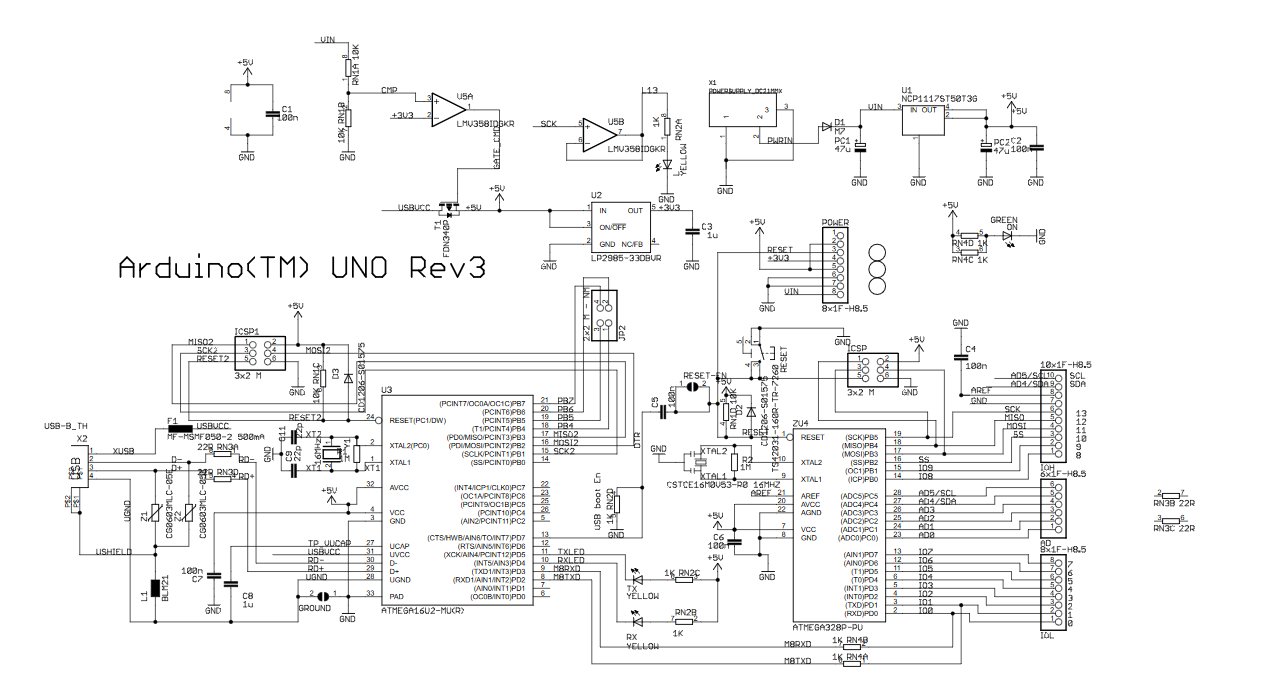
\includegraphics[width=\textwidth]{ArduinoStroomschema.png}
\end{sidewaysfigure}

\end{appendices}

\end{document}
